\documentclass[12pt, a4paper]{report}

% ============================================================
%  ENCODING E LINGUA
% ============================================================
\usepackage[utf8]{inputenc}
\usepackage[T1]{fontenc}          % Fondamentale per font europei
\usepackage[italian]{babel}

% ============================================================
%  LAYOUT E GEOMETRIA
% ============================================================
\usepackage[
    a4paper,
    top=3.5cm,
    bottom=3.5cm,
    left=2.5cm,
    right=2.5cm
]{geometry}

\usepackage{parskip}              % Spazio tra paragrafi, niente rientro
\setlength{\parindent}{0pt}       % Rientro primo paragrafo = 0

% ============================================================
%  INTESTAZIONI E PIÈ DI PAGINA
% ============================================================
\usepackage{fancyhdr}
\usepackage{lastpage}

\pagestyle{fancy}

\renewcommand{\chaptermark}[1]{\markboth{\MakeUppercase{Capitolo \thechapter}}{}}
\renewcommand{\sectionmark}[1]{\markright{\MakeUppercase{#1}}}

\fancyhf{}
\renewcommand{\headrulewidth}{0.4pt}   % Linea sottile sopra
\fancyhead[L]{\small\leftmark}         % Capitolo corrente a sinistra
\fancyhead[R]{\small\rightmark}        % Sezione corrente a destra
\fancyfoot[C]{\thepage\ di \pageref{LastPage}}  % "N di TOT" al centro

% Stile per le pagine iniziali di capitolo (plain)
\fancypagestyle{plain}{
    \fancyhf{}
    \renewcommand{\headrulewidth}{0pt}
    \fancyfoot[C]{\thepage\ di \pageref{LastPage}}
}

% ============================================================
%  TITOLI DI CAPITOLO E SEZIONE
% ============================================================
\usepackage{titlesec}
\usepackage{hyperref}

% Capitolo: numero e titolo sulla stessa riga, senza "Capitolo"
\titleformat{\chapter}[hang]
    {\normalfont\huge\bfseries}   % Formato
    {\thechapter}                 % Solo il numero
    {1em}                         % Spazio numero-titolo
    {}
\titlespacing*{\chapter}{0pt}{-20pt}{20pt}  % Riduce spazio bianco sopra

% Sezione
\titleformat{\section}
    {\normalfont\Large\bfseries}
    {\thesection}{1em}{}

% Sottosezione
\titleformat{\subsection}
    {\normalfont\large\bfseries}
    {\thesubsection}{1em}{}

% ============================================================
%  GRAFICA E FIGURE
% ============================================================
\usepackage{graphicx}
\graphicspath{{immagini/}}
\usepackage{float}
\usepackage{caption}
\usepackage{subcaption}
\usepackage{tikz}
\usetikzlibrary{shapes.geometric, arrows.meta, positioning, calc, fit, backgrounds}

\captionsetup{
    font=small,
    labelfont=bf,
    format=hang
}

% ============================================================
%  TABELLE
% ============================================================
\usepackage{booktabs}
\usepackage{tabularx}
\usepackage{longtable}

% ============================================================
%  MATEMATICA
% ============================================================
\usepackage{amsmath}
\usepackage{amssymb}

% ============================================================
%  HYPERREF (sempre ultimo)
% ============================================================
\usepackage{hyperref}
\hypersetup{
    colorlinks  = true,
    linkcolor   = black,
    citecolor   = black,
    filecolor   = black,
    urlcolor    = blue,
    pdftitle    = {Rilevamento e diagnosi dei guasti su macchinari rotanti},
    pdfauthor   = {Tempera, Marcianesi, Vianello},
    pdfsubject  = {Tesi Magistrale — UNIVPM},
    pdfkeywords = {fault detection, macchinari rotanti, machine learning}
}

% ============================================================
%  DOCUMENTO
% ============================================================
\begin{document}

% ----------------------------------------------------------
%  PAGINA DI COPERTINA
% ----------------------------------------------------------
\begin{titlepage}
    \centering

    
\includegraphics[width=0.28\textwidth]{logo}

    \vspace{0.8cm}
    {\LARGE\bfseries Università Politecnica delle Marche\par}

    \vspace{0.3cm}
    {\large Facoltà di Ingegneria\par}

    \vspace{0.2cm}
    {\normalsize Dipartimento di Ingegneria dell'Informazione\par}

    \vspace{0.8cm}
    \rule{\textwidth}{0.4pt}    % Linea separatrice superiore
    \vspace{0.4cm}

    {\large Corso di Laurea Magistrale in\\
     Ingegneria Informatica e dell'Automazione\par}

    \vspace{0.8cm}

    {\LARGE\bfseries
     Sviluppo di una Zero Trust Architecture per la gestione di un impianto di energia nucleare\par}

    \vspace{0.4cm}
    \rule{\textwidth}{0.4pt}    % Linea separatrice inferiore

    \vfill

    % Docenti e Componenti del gruppo
    \noindent
    \begin{minipage}[t]{0.48\textwidth}
        \raggedright
        {\small\textbf{Docente}}\\[4pt]
        Prof.\ Luca Spalazzi
    \end{minipage}
    \hfill
    \begin{minipage}[t]{0.48\textwidth}
        \raggedleft
        {\small\textbf{Componenti del gruppo}}\\[4pt]
        Fabio Tempera\\
        Luca Marcianesi\\
        Gabriele Vianello\\
        Gianluca Baldelli
    \end{minipage}

    \vspace{1.5cm}

    {\normalsize Anno Accademico 2025--2026\par}

\end{titlepage}

% ----------------------------------------------------------
%  INDICI
% ----------------------------------------------------------
\tableofcontents
\listoffigures
% \listoftables   % decommentare se servono tabelle

\newpage

% ----------------------------------------------------------
%  CAPITOLI
% ----------------------------------------------------------
\chapter{Introduzione}

La sicurezza informatica nei sistemi distribuiti è un campo in continua evoluzione, spinto dalla crescente complessità delle infrastrutture moderne e dall'inadeguatezza dei modelli di protezione tradizionali. Il paradigma del perimetro difensivo, in cui tutto ciò che si trova all'interno della rete aziendale è considerato affidabile per definizione, ha mostrato i propri limiti in modo sempre più evidente negli ultimi anni. Violazioni sofisticate, movimenti laterali non rilevati e compromissioni di credenziali legittime hanno reso chiaro che la fiducia implicita nella rete interna è una premessa insostenibile.

Da questa consapevolezza nasce il modello Zero Trust, la cui idea fondante può essere riassunta in un unico principio: non fidarsi mai, verificare sempre. In un'architettura Zero Trust, nessuna richiesta di accesso viene considerata sicura a priori, indipendentemente dalla provenienza, dall'identità dichiarata o dalla rete di appartenenza. Ogni accesso deve essere autorizzato esplicitamente, valutando in modo continuo il contesto dell'identità richiedente, del dispositivo utilizzato, della risorsa a cui si vuole accedere e del livello di rischio associato alla transazione.

\section{Il progetto}

Questo elaborato descrive la progettazione e l'implementazione di un'architettura Zero Trust basata su microservizi, sviluppata nell'ambito del corso di \textit{Advanced Cybersecurity for IT}. Lo scenario scelto come dominio applicativo è quello di una centrale nucleare, un contesto volutamente estremo per quanto riguarda i requisiti di sicurezza: ruoli operativi con responsabilità nettamente distinte, informazioni classificate a vari livelli di sensibilità, accesso fisico e digitale strettamente correlati e impatti potenzialmente critici in caso di compromissione.

L'architettura è distribuita su 7 componenti principali:
\begin{enumerate}
    \item PEP (Envoy PROXY)
    \item PDP (Security Orchestrator, OPA, Modello AI, Security DB)
    \item IAM 
    \item Logica (Business Logic, Business DB)
    \item Firewall
    \item IDS 
    \item SIEM (Splunk)
\end{enumerate} 
conforme ai principi definiti dalla pubblicazione NIST Special Publication 800-207, il riferimento tecnico consolidato per le implementazioni Zero Trust. Il fulcro del progetto è la separazione netta tra il Policy Enforcement Point (PEP), responsabile dell'intercettazione del traffico e dell'applicazione delle decisioni, e il Policy Decision Point (PDP), che valuta le policy e produce il verdetto di accesso. Questa separazione garantisce che nessun componente concentri in sé sia la capacità di applicare le regole sia quella di definirle, riducendo la superficie di attacco e aumentando la chiarezza architetturale.

Il sistema implementa un controllo degli accessi adattivo e basato sul rischio, che va ben oltre la semplice validazione delle credenziali. Ogni richiesta viene analizzata tenendo conto dell'impronta TLS del client tramite JA3 fingerprinting, della presenza di un certificato client valido mediante mutual TLS, dello score di anomalia restituito dal modello di ai e dalle policy di accesso definite. Il risultato è un sistema capace di prendere decisioni di accesso granulari, contestuali e dinamiche.

\section{Obiettivi}

Gli obiettivi del progetto sono articolati su più livelli. Sul piano architetturale, l'obiettivo è dimostrare come i principi Zero Trust possano essere applicati concretamente in un'infrastruttura containerizzata, con una segmentazione di rete rigorosa e una catena di autorizzazione verificabile end-to-end. Sul piano della sicurezza, si vuole mostrare come sia possibile implementare un controllo degli accessi che tenga conto simultaneamente di identità, dispositivo, rete, comportamento e classificazione della risorsa, superando i limiti dei modelli basati esclusivamente su ruoli o credenziali statiche.

Sul piano dell'osservabilità, un obiettivo esplicito è garantire la tracciabilità completa di ogni richiesta attraverso tutti i componenti del sistema, mediante la propagazione di un identificatore di correlazione univoco (\texttt{X-Request-ID}) e la centralizzazione dei log su Splunk. Tale integrazione consente sia di ricostruire il percorso di ogni transazione, sia di rilevare scenari di attacco complessi attraverso interrogazioni e allarmi configurati sulla piattaforma di monitoraggio.


\section{Struttura dell'elaborato}

L'elaborato è organizzato in modo da accompagnare il lettore dalla teoria alla pratica in modo progressivo. Il Capitolo 2 fornisce il quadro teorico completo, trattando i fondamenti della crittografia applicata, i modelli formali di controllo degli accessi, i principi di progettazione sicura e le tecnologie specifiche impiegate nel progetto. Il Capitolo 3 descrive l'architettura del sistema nei suoi componenti, flussi e scelte progettuali. Il Capitolo 4 entra nel dettaglio implementativo di ciascun modulo. Il Capitolo 5 presenta il modello di Intelligenza Artificiale di tipo Temporal Graph Network impiegato per la valutazione del rischio, descrivendone l'architettura, l'addestramento e i risultati ottenuti. Il Capitolo 6 presenta i test di carico e di sicurezza eseguiti sul sistema. Infine, il Capitolo 7 riporta le conclusioni dell'elaborato.

\chapter{Fondamenti teorici}

Prima di addentrarsi nei dettagli implementativi dell'architettura realizzata, è necessario costruire un solido quadro teorico che permetta di comprendere le scelte progettuali con piena consapevolezza del loro significato. Questo capitolo tratta i modelli formali di sicurezza, i principi di progettazione sicura, le tecnologie crittografiche alla base delle comunicazioni protette e gli strumenti specifici impiegati nel progetto.

\section{Il modello Zero Trust}

Il termine Zero Trust fu coniato da John Kindervag nel 2010, durante il suo lavoro presso Forrester Research; le radici concettuali del modello affondano tuttavia in una critica più antica al modello perimetrale. L'idea tradizionale di sicurezza informatica era quella del castello con il fossato: una rete interna considerata sicura, protetta da un perimetro difensivo verso l'esterno. Tutto ciò che si trovava all'interno del perimetro godeva di un livello implicito di fiducia. Questa assunzione si è rivelata pericolosa: una volta violato il perimetro, un attaccante poteva muoversi lateralmente attraverso la rete con scarsa resistenza.

Il modello Zero Trust rovescia questa logica in modo radicale. Nessuna entità, né utente, né dispositivo, né servizio, è considerata affidabile per default, indipendentemente dalla sua posizione nella rete. Ogni accesso deve essere esplicitamente autenticato, autorizzato e continuamente validato. La rete stessa smette di essere un elemento di fiducia e diventa semplicemente un mezzo di trasporto.

Il riferimento normativo più autorevole per l'implementazione pratica del modello è la pubblicazione NIST SP 800-207, \textit{Zero Trust Architecture}, pubblicata nel 2020. Questo documento definisce i principi fondamentali del modello e identifica i componenti logici di un'architettura Zero Trust.

\subsection{Principi fondamentali secondo NIST 800-207}

La pubblicazione NIST SP 800-207 articola il modello Zero Trust attorno a 7 principi fondamentali:

\begin{itemize}
\item tutte le risorse sono considerate non affidabili, indipendentemente dalla loro posizione nella rete;
\item tutte le comunicazioni devono essere protette, anche quelle interne alla rete aziendale;
\item l'accesso alle risorse deve essere concesso su base per-sessione e con il minimo privilegio necessario;
\item l'accesso è determinato da policy dinamiche che tengono conto dell'identità, del dispositivo, della rete e di altri attributi contestuali;
\item l'integrità e la sicurezza di tutti i dispositivi connessi devono essere monitorate e verificate;
\item l'autenticazione e l'autorizzazione devono essere eseguite in modo dinamico e rigoroso prima di consentire l'accesso;
\item l'organizzazione deve raccogliere quante più informazioni possibile sullo stato delle risorse e delle comunicazioni, e usarle per migliorare continuamente la postura di sicurezza.
\end{itemize}

\subsection{Policy Enforcement Point e Policy Decision Point}

L'architettura Zero Trust secondo NIST si articola attorno a 2 componenti logici principali. Il Policy Enforcement Point (PEP) è il punto in cui il traffico viene intercettato e le decisioni di accesso vengono applicate. Il PEP non decide autonomamente: riceve un verdetto da un'entità separata e lo esegue, consentendo o bloccando la richiesta. Il Policy Decision Point (PDP) è invece il componente che valuta le policy e produce il verdetto. Nel modello NIST, il PDP si compone a sua volta di un Policy Engine, che applica le regole di accesso, e di un Policy Administrator, che traduce il verdetto in istruzioni operative per il PEP.

La separazione tra PEP e PDP è un requisito architetturale fondamentale, non una mera convenzione. Essa garantisce che la logica di applicazione delle regole e la logica di definizione delle regole siano mantenute distinte, riducendo la complessità di ciascun componente e limitando il raggio di impatto di una potenziale compromissione.

Nel progetto descritto in questo elaborato, il PEP è implementato da Envoy Proxy, mentre il PDP è realizzato dalla combinazione del Security Orchestrator, del modello di AI e dal motore di policy OPA.

\section{Modelli formali di controllo degli accessi}
\label{sec:Modelli formali di controllo degli accessi}

La teoria del controllo degli accessi ha radici che risalgono agli anni Settanta e ha prodotto modelli formali che ancora oggi informano la progettazione dei sistemi di sicurezza moderni. Comprendere questi modelli è essenziale per valutare le scelte architetturali di qualsiasi sistema che gestisca risorse con livelli di sensibilità differenziati.

\subsection{Controllo degli accessi basato su ruoli}

Il Role-Based Access Control (RBAC), standardizzato nella pubblicazione ANSI/INCITS 359-2004, è un modello di controllo degli accessi in cui i permessi non sono assegnati direttamente agli utenti ma ai ruoli, e gli utenti acquisiscono i permessi in virtù dell'appartenenza a uno o più ruoli. Il riferimento NIST specifico per RBAC è invece la pubblicazione NIST IR 7316, che definisce le specifiche funzionali del modello senza costituire essa stessa lo standard ANSI/INCITS. Questo approccio semplifica notevolmente la gestione degli accessi in sistemi con molti utenti e molte risorse.

Nel progetto il modello Role-Based Access Control costituisce il livello di base per l'astrazione e la gestione delle identità all'interno del sistema di autorizzazione. A differenza delle implementazioni RBAC tradizionali, dove il ruolo determina staticamente i permessi di accesso a specifiche risorse, in questa architettura il ruolo funge da livello di disaccoppiamento organizzativo.
Le identità degli utenti vengono veicolate tramite token JWT dai quali viene estratto un attributo di business (ad esempio: \texttt{guest}, \texttt{operator}, \texttt{manager}, \texttt{admin}). Il motore di policy utilizza una mappa associativa per convertire questi ruoli organizzativi in etichette di sicurezza. 

Invece di assegnare individualmente complessi set di parametri ad ogni singolo dipendente, l'appartenenza a un ruolo popola dinamicamente gli attributi strutturali necessari ai modelli successivi.

\subsection{Controllo degli accessi basato su attributi}

Il modello Attribute-Based Access Control (ABAC) estende RBAC introducendo la valutazione di attributi arbitrari relativi al soggetto, alla risorsa, all'ambiente e all'azione richiesta. Le decisioni di accesso non dipendono solo dal ruolo dell'utente, ma da una combinazione di attributi che può includere l'ora della richiesta, il tipo di dispositivo, il livello di rischio corrente e qualsiasi altra informazione contestuale rilevante.

Nell'implementazione realizzata, l'approccio ABAC permette di superare i limiti di un'autorizzazione puramente statica valutando il contesto di ogni singola richiesta in tempo reale. Agli attributi dell'oggetto (come il percorso specifico dell'endpoint e il metodo HTTP) vengono associati metadati quantitativi intrinseci di rischio. 

L'elemento architetturale chiave introdotto in questa fase è la valutazione degli attributi ambientali, rappresentati specificamente da uno \textit{score di rischio} continuo. Attraverso questo scambio di attributi, l'ABAC realizza concretamente il principio della valutazione continua del rischio.

\subsection{Il modello Bell-LaPadula}

Il modello Bell-LaPadula, proposto da David Elliott Bell e Leonard J. LaPadula nel 1973 per conto della United States Air Force, è il modello formale di riferimento per la confidenzialità delle informazioni. Il suo obiettivo è impedire che informazioni riservate fluiscano verso soggetti non autorizzati a riceverle.

Il modello introduce il concetto di livello di sicurezza, originariamente costituito da 2 dimensioni che formano una struttura a reticolo: una gerarchia totalmente ordinata e un insieme non gerarchico di compartimenti o categorie. Nel progetto realizzato, i livelli gerarchici adottati sono 5: PUBLIC, INTERNAL, CONFIDENTIAL, SECRET e TOP\_SECRET, in ordine crescente di sensibilità. A questi si affiancano specifiche categorie (es. \textit{nuclear, security}). Un accesso è consentito solo se, oltre a soddisfare i vincoli di livello, il soggetto possiede un insieme di categorie che include (superset) tutte quelle richieste dall'oggetto.

Il modello formale completo si fonda su 3 proprietà fondamentali del Mandatory Access Control (MAC). La \textit{Simple Security Property} (o proprietà \textit{no read-up}) stabilisce che un soggetto può leggere un oggetto solo se il suo livello di autorizzazione domina quello dell'oggetto. La \textit{Star Property} (o proprietà \textit{no write-down}) stabilisce che un soggetto non può scrivere su un oggetto con livello di classificazione inferiore al proprio, impedendo il declassamento illecito delle informazioni. La terza proprietà, la \textit{Discretionary Security Property} (ds-property), regola gli accessi discrezionali tramite una matrice degli accessi sovrapposta al controllo obbligatorio basato sui livelli: un soggetto può accedere a un oggetto solo se, oltre a soddisfare le 2 proprietà precedenti, la matrice degli accessi discrezionali autorizza esplicitamente quella particolare combinazione di soggetto, oggetto e modalità di accesso. Il progetto implementa le prime 2 proprietà; la ds-property non è oggetto di un'implementazione dedicata, costituendo una lacuna teorica rispetto alla formulazione completa del modello.

\subsubsection{Esempio di sanificazione}
Tuttavia, l'implementazione in OPA estende questo concetto introducendo la figura del \textit{Trusted Subject}: viene definita una deroga controllata alla \textit{Star Property} per consentire a un utente \texttt{admin} (TOP\_SECRET) di scrivere su una specifica rotta sanitizzata di livello inferiore (SECRET), permettendo così una de-classificazione sicura delle informazioni.

\begin{figure}[h]
    \centering
    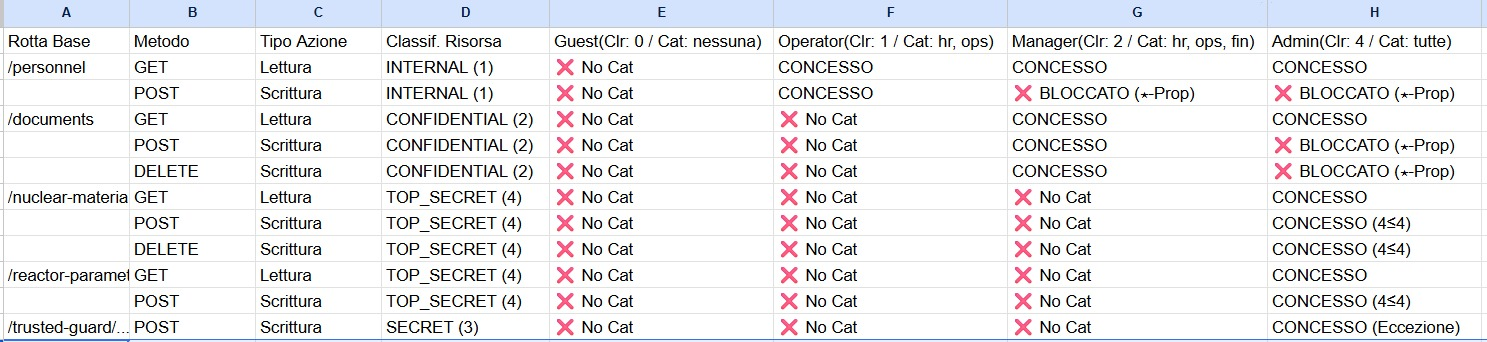
\includegraphics[width=0.9\textwidth]{immagini/bell-lapadula.jpeg}
    \caption{Tabella Bell\-Lapadula}
    \label{fig:BellLapadula}
\end{figure}

\subsection{Algoritmo di fiducia}

L'algoritmo di fiducia implementato nel file \texttt{policy.rego} di OPA si distingue per la sua architettura \textit{ibrida}, che fonde metodologie di controllo rigido degli attributi (tipiche dei sistemi Mandatory Access Control) con meccanismi di controllo basato sul punteggio.

\subsubsection{Controllo degli Attributi: Modello Bell-LaPadula}
La componente deterministica dell'algoritmo si basa su un'implementazione del modello di confidenzialità Bell-LaPadula (BLP).
\subsubsection{Controllo basato sul punteggio: valutazione dinamica del rischio}
A valle del controllo deterministico, l'algoritmo ibrido introduce una fase di computazione algoritmica basata sulla somma e sottrazione di attributi di rischio continuo. Questo garantisce che credenziali compromesse (ma formalmente valide nel modello BLP) non siano sufficienti per finalizzare un attacco.

Per ogni singola richiesta HTTP, l'algoritmo valuta:
\begin{itemize}
    \item \textit{beneficio dell'operazione} ($B$): un indice quantitativo pre-assegnato al metodo e alla rotta (es. $0.9$ per rotte critiche, $0.6$ per risorse interne);
    \item \textit{punteggio AI di minaccia} ($A$): un attributo dinamico valutato in tempo reale che quantifica il livello di rischio della richiesta.
    \item \textit{beneficio netto}: \begin{equation}
    B_{netto} =  B - A \end{equation}
    \item \textit{soglia di beneficio netto minimo} ($B_{m}$): il livello minimo di beneficio netto richiesto per la specifica transazione(es. $0.8$ per rotte critiche, $0.3$ per risorse interne);
\end{itemize}

Il blocco di autorizzazione finale si risolve tramite la disuguaglianza algebrica :
\begin{equation}
    B - A \geq B_{m}
\end{equation}
Questa disuguaglianza impone che un'operazione venga completata unicamente se il suo vantaggio contestuale eccede la soglia di beneficio netto minimo richiesto configurato per lo specifico endpoint. È importante chiarire la semantica di $B$ per evitare un'interpretazione fuorviante: il parametro non misura la sensibilità o criticità della risorsa, ma il beneficio operativo, cioè quanto è necessario che l'operazione vada a buon fine per il corretto funzionamento del sistema (ad esempio, un'operazione di lettura su una rotta di monitoraggio essenziale per la sicurezza dell'impianto può avere beneficio più alto di una scrittura su una risorsa interna non urgente, indipendentemente dalla classificazione di sensibilità del dato). Il parametro che effettivamente codifica la criticità della risorsa è $B_{m}$: alle rotte più sensibili viene assegnata una soglia di beneficio netto minimo accettato molto più alta, cosicché anche un beneficio numerico elevato non comprometta la sicurezza complessiva, poiché la disuguaglianza richiede comunque che il punteggio di rischio AI resti contenuto entro un margine ristretto. I due parametri sono quindi calibrati congiuntamente per ciascuna rotta, e non in modo indipendente: un beneficio alto su una rotta critica è sempre accompagnato da una soglia di beneficio netto minimo accettato proporzionalmente più severa.


\section{Principi di progettazione sicura}

Parallelamente ai modelli formali, la letteratura di sicurezza informatica ha elaborato un insieme di principi di progettazione che guidano la costruzione di sistemi resistenti. Questi principi, enunciati originariamente da Jerome Saltzer e Michael Schroeder nel loro articolo seminale del 1975 \textit{The Protection of Information in Computer Systems}, rimangono di piena attualità e informano ogni scelta architetturale significativa.

\subsection{Economy of mechanism}

Il principio di economy of mechanism afferma che i meccanismi di sicurezza devono essere progettati per essere il più semplici e piccoli possibile. La semplicità riduce la probabilità di errori implementativi, semplifica la verifica della correttezza e limita la superficie di attacco. Un meccanismo complesso è più difficile da capire, da testare e da mantenere nel tempo.

Nel progetto, questo principio si manifesta nella scelta di componenti con responsabilità ben definite e limitate. nftables si occupa esclusivamente del filtraggio del traffico a livello di rete, Envoy gestisce la terminazione TLS e la delega dell'autorizzazione, OPA valuta le policy in linguaggio Rego: ciascuno di questi componenti rispetta pienamente il principio.

\subsection{Fail-safe defaults}

Il principio di fail-safe defaults stabilisce che, in assenza di una decisione di autorizzazione esplicita, il sistema deve negare l'accesso. Il comportamento predefinito deve essere il rifiuto, non il consenso. Un sistema che fallisce in modo sicuro limita i danni derivanti da errori di configurazione o da condizioni impreviste.

Questo principio è visibile in più punti dell'architettura. La policy OPA definisce \texttt{default allow = false}, garantendo che qualsiasi richiesta per cui non sia applicabile una regola esplicita di consenso venga negata automaticamente. Analogamente, la catena di nftables configura la policy di default del chain \texttt{input} a DROP, in modo che solo il traffico esplicitamente consentito possa raggiungere il sistema.

\subsection{Complete mediation}

Il principio di complete mediation afferma che ogni accesso a ogni risorsa deve essere verificato, senza eccezioni e senza possibilità di aggirare il meccanismo di controllo. Non deve esistere alcun percorso che consenta di accedere a una risorsa senza passare attraverso il punto di autorizzazione.

L'architettura del progetto garantisce la complete mediation attraverso la topologia di rete. Il Business DB, che contiene i dati più sensibili dell'applicazione, è raggiungibile esclusivamente dal servizio Business Logic attraverso la rete isolata Back-Net. Ogni richiesta al servizio applicativo deve necessariamente transitare per Envoy, che intercetta il traffico e delega l'autorizzazione prima di instradare la richiesta. Come descritto nel Capitolo 3, non esiste alcun percorso diretto dall'esterno, dal Security Orchestrator o dal motore PDP verso il Business DB: nessuno dei componenti del piano decisionale dispone di credenziali proprie su tale database, e l'unico punto di accesso resta il servizio Business Logic attraverso la rete isolata Back-Net.

\subsection{Separation of privilege}

Il principio di separation of privilege afferma che un sistema non dovrebbe concedere l'accesso o eseguire un'operazione sulla base di un'unica condizione, ma richiedere la soddisfazione di più condizioni indipendenti. La separazione dei privilegi riduce il rischio che la compromissione di un singolo fattore sia sufficiente a violare la sicurezza del sistema.

Nel progetto, la decisione di accesso richiede la soddisfazione simultanea di più condizioni: l'utente deve avere un livello di clearance adeguato alla classificazione della risorsa, un trust score superiore alla soglia minima richiesta dalla zona, l'enrollment MFA dove richiesto, un dispositivo di tipo consentito e una provenienza di rete autorizzata. La compromissione di un solo fattore, ad esempio il furto di credenziali, non è sufficiente a ottenere l'accesso se il dispositivo utilizzato non corrisponde all'impronta JA3 attesa o se il trust score è al di sotto della soglia.

\subsection{Least privilege}

Il principio del minimo privilegio afferma che ogni entità del sistema, utente, processo o componente, deve operare con il minimo insieme di permessi necessario per svolgere le proprie funzioni. Questo limita i danni in caso di compromissione e riduce la superficie di attacco disponibile.

L'applicazione di questo principio è pervasiva nell'architettura. Il servizio Business Logic non si connette al database con un'unica utenza a privilegi globali, ma utilizza 3 credenziali MongoDB distinte e role-scoped (\texttt{operator\_client}, \texttt{manager\_client}, \texttt{admin\_client}), ciascuna abilitata alle sole collection pertinenti al rispettivo livello. In questo modo il principio del minimo privilegio è applicato non solo dalla policy di autorizzazione, ma anche dalle credenziali con cui si raggiunge effettivamente il dato, fornendo un secondo strato di difesa indipendente. Ogni microservizio, analogamente, opera all'interno del segmento di rete strettamente necessario alle proprie funzioni.

\subsection{Open design}

Il principio di open design afferma che la sicurezza di un sistema non deve dipendere dalla segretezza del suo meccanismo di protezione, ma esclusivamente dalla segretezza delle chiavi o delle credenziali. Un sistema la cui sicurezza dipende dall'oscurità della propria implementazione risulta strutturalmente debole: qualora il meccanismo venga scoperto, l'efficacia della protezione viene del tutto compromessa.

Nel progetto, i meccanismi di protezione sono basati su standard aperti e ampiamente verificati: TLS 1.3 per la cifratura delle comunicazioni, X.509 per i certificati, SHA-256 per gli hash di integrità. La sicurezza risiede nella segretezza delle chiavi private, non nella segretezza degli algoritmi. Le policy OPA sono espresse in Rego, un linguaggio leggibile e auditabile, la cui correttezza può essere verificata in modo indipendente; il documento non include tuttavia il codice Rego della policy né nel corpo del testo né in appendice, il che rende di fatto impossibile per il lettore verificare l'affermazione di auditabilità sulla base del materiale presentato.

\subsection{Psychological acceptability}

Il principio di psychological acceptability afferma che i meccanismi di sicurezza devono essere progettati in modo da non creare ostacoli eccessivi agli utenti legittimi. Se i controlli di sicurezza sono troppo onerosi, gli utenti troveranno modi per aggirarli. La sicurezza deve essere praticabile, non solo teoricamente corretta.

In un'architettura Zero Trust, questo principio si traduce nella trasparenza dei controlli: l'autenticazione e l'autorizzazione avvengono in modo il più possibile automatico, senza richiedere azioni aggiuntive all'utente se non nei casi in cui il rischio lo giustifichi. Nell'implementazione realizzata, tuttavia, l'autenticazione a più fattori è richiesta a ogni singolo login, indipendentemente dal livello di rischio della sessione: dopo la verifica di username e password, il sistema emette sempre un codice OTP monouso inviato via email che l'utente deve confermare prima che venga rilasciato il token di sessione. Questa scelta è in tensione diretta con il principio appena enunciato, che prevede l'introduzione di attriti aggiuntivi solo quando il rischio lo giustifica e non in modo incondizionato; va inoltre osservato che l'OTP via email è generalmente considerato in letteratura un secondo fattore relativamente debole, una caratteristica rilevante per un sistema che protegge un impianto nucleare.

\section{Crittografia applicata e TLS}

Le comunicazioni sicure all'interno dell'architettura si fondano su protocolli crittografici standard. La comprensione dei meccanismi sottostanti è necessaria per valutare le garanzie di sicurezza offerte dal sistema.

\subsection{Transport Layer Security}

Il protocollo TLS (Transport Layer Security) è lo standard de facto per la protezione delle comunicazioni su reti non affidabili. La versione corrente, TLS 1.3, definita nella RFC 8446, introduce significativi miglioramenti rispetto alle versioni precedenti: eliminazione di suite crittografiche deboli, riduzione della latenza dell'handshake da 2 round-trip a uno, e forward secrecy obbligatoria attraverso l'uso esclusivo di scambi di chiave effimeri basati su Diffie-Hellman.

Il processo di handshake TLS stabilisce un canale sicuro tra client e server attraverso una sequenza di messaggi che negozia le suite crittografiche, autentica le parti e deriva le chiavi di sessione. Il risultato è un canale che garantisce confidenzialità (attraverso la cifratura simmetrica), integrità (attraverso MAC o AEAD) e autenticazione (attraverso certificati digitali). È opportuno precisare che la forward secrecy obbligatoria di TLS 1.3 riguarda esclusivamente le chiavi di sessione, derivate in modo effimero a ogni handshake: i certificati client statici impiegati nel mutual TLS non beneficiano direttamente di questa proprietà, poiché la chiave privata associata al certificato resta fissa nel tempo. La compromissione di tale chiave privata, pur non esponendo le sessioni passate già concluse, comprometterebbe comunque l'autenticazione futura del client fino alla revoca o al rinnovo del certificato.

Nel progetto, Envoy termina le connessioni TLS in ingresso, gestendo il processo di handshake e l'estrazione dei metadati crittografici attraverso il TLS Inspector. L'uso di TLS 1.3 è rilevante anche per il JA3 fingerprinting: client che negoziano con cipher suite o versioni TLS datate producono hash JA3 distinti e riconoscibili, consentendo al sistema di identificare connessioni anomale anche in presenza di credenziali valide.

\subsection{Mutual TLS}

Il mutual TLS (mTLS) è un'estensione del protocollo TLS in cui entrambe le parti, client e server, si autenticano reciprocamente mediante certificati digitali X.509. Nel TLS standard, solo il server presenta un certificato per autenticarsi al client; nell'mTLS, anche il client è tenuto a presentare un certificato valido, firmato da una Certificate Authority (CA) fidata dal server.

Questo meccanismo è particolarmente adatto agli ambienti Zero Trust, perché fornisce un'autenticazione forte basata su crittografia a chiave pubblica, indipendente da credenziali riutilizzabili come username e password. Un client che non disponga di un certificato valido firmato dalla CA interna non può stabilire una connessione, indipendentemente da qualsiasi altra credenziale. Va segnalato che il progetto non prevede alcun meccanismo di revoca dei certificati, né tramite Certificate Revocation List (CRL) né tramite Online Certificate Status Protocol (OCSP): in un'architettura Zero Trust la capacità di revocare rapidamente un certificato compromesso costituisce un requisito fondamentale, che in questo caso resta privo di copertura. Una mitigazione parziale, non implementata nella versione corrente del progetto ma proponibile come lavoro futuro, consisterebbe nell'adozione di certificati a vita molto breve (short-lived certificates, tipicamente con validità di ore) rilasciati da una CA interna automatizzata: questo approccio, diffuso in architetture Zero Trust moderne, riduce drasticamente la finestra di esposizione di un certificato compromesso senza richiedere l'infrastruttura aggiuntiva di un servizio CRL o OCSP, spostando di fatto il problema della revoca verso quello, più gestibile, del rinnovo automatico frequente.

Nel progetto, Envoy è configurato con \texttt{require\_client\_certificate: false}, rendendo facoltativa la presentazione di un certificato client firmato dalla CA interna. I certificati sono generati tramite OpenSSL con il parametro di estensione \texttt{extendedKeyUsage=client Auth}, garantendo che possano essere utilizzati esclusivamente per l'autenticazione del client. Al termine dell'handshake, quando un certificato è presente, Envoy ne inietta i metadati nell'header \texttt{X-Forwarded-Client-Cert}; il Security Orchestrator li interpreta per risolvere l'identità del soggetto richiedente in modo crittograficamente verificato e li inoltra al livello di policy. Questa configurazione è in tensione con la filosofia Zero Trust dichiarata per il progetto: rendere facoltativo il certificato a livello TLS significa demandare per intero la verifica al Security Orchestrator e, più a valle, al servizio Identity (si veda la discussione al Capitolo 3 e alla Sezione~\ref{sec:autenticazionestandard}), introducendo un punto di fiducia implicita su Envoy. Sebbene il controllo applicativo successivo blocchi correttamente le richieste prive di certificato per i ruoli che lo richiedono, l'assenza di enforcement a livello di trasporto resta una scelta architetturale che meriterebbe un'analisi critica più esplicita nel documento, dato che espone comunque superficie applicativa a un client non ancora autenticato a livello TLS.

\subsection{JA3 fingerprinting}

Il JA3 fingerprinting è una tecnica di identificazione del client basata sui parametri dell'handshake TLS. Sviluppata da John Althouse, Jeff Atkinson e Josh Atkins presso Salesforce nel 2017, costruisce una firma identificativa del client a partire da 5 campi dell'handshake: la versione TLS proposta, le cipher suite supportate, le estensioni TLS incluse, i gruppi di curve ellittiche e i formati di punto ellittico.

Questi 5 campi vengono concatenati in una stringa con separatori definiti e poi sottoposti a hashing MD5, producendo un identificatore di 32 caratteri esadecimali che è caratteristico della combinazione di libreria TLS e configurazione utilizzata dal client. Client diversi, anche se usano le stesse credenziali, produrranno hash JA3 differenti se il loro stack TLS è diverso. Questo rende il JA3 uno strumento utile per rilevare impersonificazioni, bot e client anomali anche quando le credenziali presentate sono valide. La tecnica presenta tuttavia limiti ben noti che il progetto non affronta esplicitamente: un tasso di collisione non trascurabile tra client diversi che condividono la stessa libreria e versione TLS, la possibilità di spoofing intenzionale dell'impronta da parte di un attaccante che ne conosca i parametri di calcolo, e una progressiva perdita di efficacia con l'adozione di TLS 1.3, dove la riduzione della variabilità osservabile dell'handshake limita la distintività delle impronte, fino all'inutilizzabilità completa quando il client adotta l'estensione Encrypted Client Hello (ECH), che cifra interamente i parametri dell'handshake altrimenti usati per il calcolo del fingerprint.

Nel progetto, Envoy è configurato con \texttt{enable\_ja3\_fingerprinting: true} nel filtro TLS Inspector. Envoy espone la stringa JA3 grezza come variabile di metadato e la inietta negli header della richiesta inoltrata al Security Orchestrator. È quest'ultimo a calcolarne il digest MD5, ottenendo l'hash a 32 caratteri esadecimali.

\section{Componenti tecnologici}

\subsection{nftables}

nftables è il framework di filtraggio dei pacchetti del kernel Linux, introdotto come successore di iptables a partire dal kernel 3.13. A differenza di iptables, nftables offre una sintassi unificata per IPv4 e IPv6, supporto nativo per set e mappe di indirizzi, e un'architettura interna più efficiente basata su una macchina virtuale integrata nel kernel.

Nel progetto, nftables opera come firewall di rete posizionato tra il client esterno e il
  resto dell'infrastruttura. La sua configurazione definisce una tabella \texttt{inet filter} le
  cui 3 catene principali, \texttt{input}, \texttt{forward} e \texttt{output}, adottano tutte
  una policy di default DROP, così che solo il traffico esplicitamente consentito venga
  accettato in ciascuna direzione. In particolare la catena \texttt{output} ammette il solo
  traffico in uscita strettamente necessario, ossia la risoluzione DNS e la comunicazione verso
  i microservizi interni. La catena \texttt{input} accetta il traffico locale, il traffico
  appartenente a connessioni già stabilite e il traffico TCP verso la porta di Envoy da
  indirizzi non presenti nella lista di blocco, loggando ogni pacchetto accettato o rifiutato
  tramite il gruppo NFLOG 100.

\subsection{Snort}

Snort è un sistema di rilevamento e prevenzione delle intrusioni di rete (NIDS/NIPS) open source, originariamente sviluppato da Marty Roesch nel 1998 e successivamente acquisito da Cisco. Opera analizzando il traffico di rete in tempo reale, confrontando i pacchetti catturati con un insieme di regole configurabili per rilevare pattern corrispondenti ad attività malevole note.

Snort può operare in 3 modalità: sniffer (stampa i pacchetti sulla console), packet logger (salva i pacchetti su disco) e network intrusion detection system (analizza i pacchetti e genera alert). Nel progetto, Snort è configurato in modalità NIDS con output su console, condivide lo stack di rete del container firewall tramite la direttiva \texttt{network\_mode: service:firewall}, e monitora l'interfaccia eth0.

La regola custom configurata utilizza il preprocessore \texttt{sfportscan} per rilevare scansioni di porte, abilitato con il parametro \texttt{sense\_level: low} per minimizzare i falsi positivi. Una regola Snort aggiuntiva segnala esplicitamente la rilevazione di un port scan TCP quando vengono rilevati più di 5 pacchetti SYN dalla stessa sorgente nell'arco di 5 secondi. Questo scenario è uno dei vettori di attacco testati esplicitamente nel progetto, con client di test che simulano la scansione rapida di un intervallo di porte.

\subsection{Envoy Proxy}

Envoy è un proxy L4/L7 open source sviluppato originariamente da Lyft e successivamente donato alla Cloud Native Computing Foundation (CNCF). È progettato per essere il piano dati di architetture a microservizi, gestendo la comunicazione tra servizi con funzionalità avanzate di load balancing, circuit breaking, osservabilità e sicurezza.

Nel contesto del progetto, Envoy svolge il ruolo di Policy Enforcement Point. La sua configurazione YAML definisce un listener sulla porta 8443 che, grazie al filtro \texttt{tls\_inspector}, ispeziona i parametri dell'handshake TLS prima ancora che la connessione sia completamente stabilita. Il filtro \texttt{http\_connection\_manager} gestisce la connessione HTTP una volta che l'handshake TLS è concluso. Envoy è configurato per richiedere il certificato client e per loggare in formato JSON strutturato una serie di informazioni sulla connessione, tra cui la versione TLS, la cipher suite, l'indirizzo remoto e l'hash JA3, propagando l'header \texttt{X-Request-ID} per garantire la tracciabilità.

Il protocollo \texttt{ext\_authz} di Envoy permette di delegare la decisione di autorizzazione a un servizio esterno, in questo caso il Security Orchestrator, prima di instradare la richiesta verso il backend. Questo è il meccanismo attraverso cui si realizza la separazione tra PEP e PDP.

\subsection{Open Policy Agent e Rego}

Open Policy Agent (OPA) è un motore di policy general-purpose open source, mantenuto dalla CNCF, che permette di esprimere e valutare policy in modo unificato attraverso diversi domini applicativi. OPA riceve in input un documento JSON che rappresenta il contesto della richiesta e valuta le policy scritte in Rego, restituendo un documento JSON che rappresenta la decisione.

Rego è un linguaggio dichiarativo derivato da Datalog, progettato specificamente per la definizione di policy. A differenza di un linguaggio imperativo, in Rego si descrive \textit{cosa} deve essere vero perché una policy sia soddisfatta, non \textit{come} verificarlo. Questo rende le policy leggibili, componibili e verificabili in modo indipendente rispetto al codice applicativo che le esegue.

Nel progetto, OPA opera come Policy Decision Point puro. Riceve dall'Orchestratore un payload che contiene ruolo dell'utente, risorsa richiesta, metodo e score del rischio generato dal modello di AI. OPA valuta tutte queste condizioni, come descritto in precedenza nella \autoref{sec:Modelli formali di controllo degli accessi}, restituendo un verdetto binario allow/deny. La separazione tra la policy e il codice che la applica garantisce che le regole possano essere modificate, testate e verificate in modo indipendente dalla logica applicativa.

\subsection{Splunk}

Splunk è una piattaforma di analisi operativa dei dati macchina, ampiamente utilizzata come SIEM (Security Information and Event Management) in ambito enterprise. Raccoglie log da sorgenti eterogenee, li normalizza, li indicizza e li rende ricercabili e correlabili attraverso il linguaggio di query SPL (Search Processing Language).

Nel progetto, Splunk opera come centro di osservabilità dell'intera architettura. Ogni microservizio invia i propri log a Splunk tramite l'HTTP Event Collector (HEC), un endpoint HTTP che accetta eventi in formato JSON autenticati tramite token. L'uso del formato JSON strutturato permette a Splunk di indicizzare automaticamente i campi dei log, rendendoli immediatamente disponibili per ricerche e correlazioni.

Il campo \texttt{X-Request-ID}, propagato da Envoy e ripreso da ogni microservizio lungo la catena di elaborazione, è il meccanismo fondamentale per la correlazione degli eventi. Dato un identificatore di richiesta, è possibile ricostruire in Splunk il percorso completo della transazione attraverso tutti i componenti: il log del firewall nftables, il log di accesso di Envoy con l'hash JA3 e il codice di risposta, il log del Security Orchestrator con l'esito della valutazione OPA e le eventuali ragioni di deny, e il log del servizio di Business Logic.

\subsection{MongoDB}

MongoDB è un database orientato ai documenti, appartenente alla famiglia NoSQL, che archivia i dati in formato BSON (Binary JSON). La sua flessibilità dello schema e il supporto nativo per documenti annidati lo rendono particolarmente adatto a modellare strutture dati eterogenee e ricche di contesto come quelle richieste da un'architettura Zero Trust.

Nel progetto sono presenti 2 istanze MongoDB con ruoli distinti. Il Security DB conserva i
  dati di identità e dispositivo gestiti dall'iam-service e dal Security Orchestrator: le
  credenziali degli utenti con ruolo, livello di clearance e flag di enrollment TPM (collection
  \texttt{identity\_users}), le credenziali WebAuthn\/FIDO2 dei dispositivi registrati
  (\texttt{device\_fingerprints}), lo stato effimero delle sessioni OTP
  (\texttt{otp\_sessions}), la blocklist dei token JWT revocati (\texttt{jwt\_blocklist}), lo
  storico immutabile degli eventi di autenticazione (\texttt{auth\_events}) e i contatori per il
  rate limiting (\texttt{rate\_limits}). Il Business DB archivia i dati applicativi della
  centrale nucleare, organizzati in 7 collection: personnel, access-badges, zones,
  reactor-parameters, maintenance-orders, documents e nuclear-materials.

\subsection{Docker e Docker Compose}

Docker è una piattaforma di containerizzazione che permette di eseguire applicazioni in ambienti isolati e riproducibili. Ogni container condivide il kernel del sistema operativo host ma dispone di un proprio filesystem, spazio di rete e namespace di processi, garantendo un isolamento sufficiente per la segmentazione dei microservizi.

  Docker Compose è lo strumento di orchestrazione usato per definire e gestire l'insieme dei
  container che compongono l'applicazione. Il file \texttt{docker-compose.yaml} del progetto
  definisce 17 servizi: oltre ai componenti principali dell'architettura
  (\texttt{firewall}, \texttt{envoy}, \texttt{security-orchestrator}, \texttt{opa} e
  \texttt{business-logic}), comprende le 3 istanze di rilevamento delle intrusioni
  (\texttt{snort}, \texttt{snort-internal} e \texttt{snort-mid}), il servizio di identità
  \texttt{iam-service} con il relativo server di posta di sviluppo \texttt{mailhog}, il
  microservizio di scoring \texttt{ai-inference}, i 2 database \texttt{business-db} e
  \texttt{security-db}, l'utility \texttt{seeder}, lo stack di osservabilità (\texttt{splunk}
  con l'universal forwarder \texttt{splunk-uf}) e il generatore di alert di test
  \texttt{alerts-tester}. La topologia di rete è definita attraverso 4 reti Docker
  isolate: Front-Net, che collega i client al firewall e al Security Orchestrator; Auth-Net, che
  connette il Security Orchestrator a OPA, al servizio di identità e alla Security DB;
  Back-Net, che connette esclusivamente Business Logic e Business DB; e Snort-Net, dedicata al
  trasporto degli alert dalle istanze Snort verso il Security Orchestrator. Questa segmentazione
  garantisce che nessun componente possa comunicare direttamente con un servizio al di fuori
  del proprio segmento di rete autorizzato, applicando la complete mediation a livello
  infrastrutturale.

\subsection{Go}

Go, o Golang, è un linguaggio di programmazione compilato e tipizzato staticamente, sviluppato da Google e rilasciato nel 2009. Le sue caratteristiche principali includono la semplicità del modello di concorrenza basato su goroutine e canali, la produzione di binari staticamente linkati senza dipendenze runtime, e una libreria standard ricca che include primitive per la gestione di connessioni TCP, HTTP e TLS.

I servizi applicativi del progetto, Security Orchestrator e Business Logic, sono scritti in Go. Le linee guida di sviluppo interne al progetto prescrivono la propagazione del contesto tramite \texttt{context.Context} in tutte le chiamate che coinvolgono I/O, il wrapping degli errori con \texttt{fmt.Errorf} per preservare la traccia completa, e l'inclusione del \texttt{X-Request-ID} in tutti i log per garantire la tracciabilità. I client di test, scritti sia in Go sia in Python, simulano scenari di accesso legittimo, accesso anomalo con cipher suite deprecate e scansione delle porte, fornendo la base per la validazione dell'architettura.

\chapter{Architettura del sistema}

L'architettura di ZTALeaks si fonda su un principio fondamentale: nessun elemento interno riceve fiducia implicita e ogni componente opera con responsabilità rigidamente confinate. Il sistema implementa concretamente la separazione tra Policy Enforcement Point (PEP) e Policy Decision Point (PDP) prescritta dalle linee guida dello standard NIST SP 800-207. Questa separazione viene realizzata tramite un ecosistema di microservizi isolati a livello di rete e containerizzati, i quali cooperano attraverso scambi protetti e log tracciabili in modo centralizzato.

\begin{figure}[h]
    \centering
    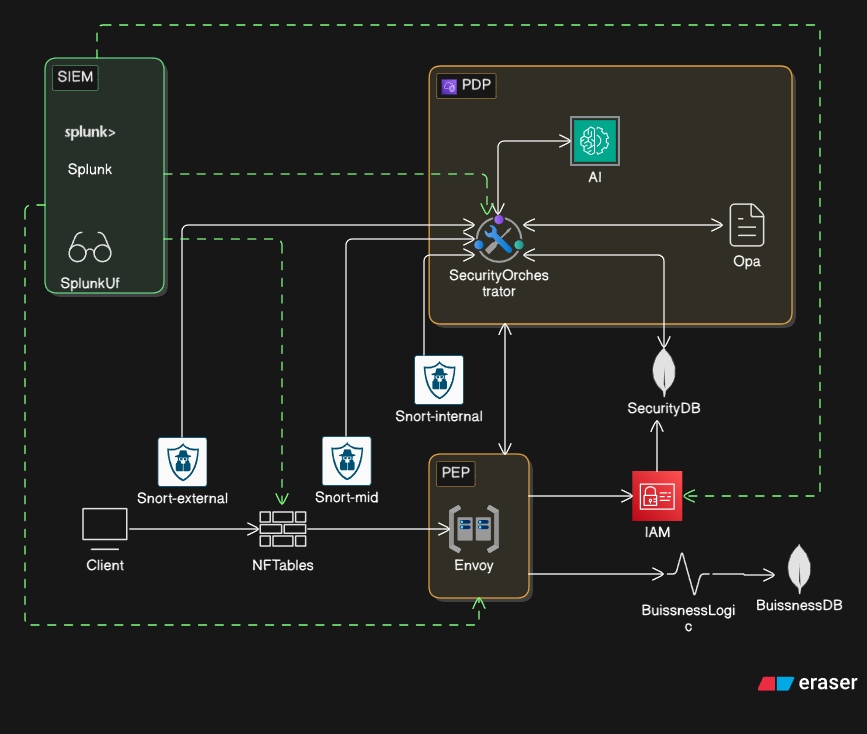
\includegraphics[width=0.7\textwidth]{immagini/architettura.png}
    \caption{Immagine architettura}
    \label{fig:immagine}
\end{figure}

\section{Struttura della repository}

Il codice sorgente dell'infrastruttura è strutturato per rispecchiare la scomposizione logica del sistema. Le cartelle principali che compongono il progetto sono descritte nell'elenco seguente:

\begin{itemize}
\item \texttt{api/}: ospita il contratto protocollare \texttt{ext\_authz.proto}, che costituisce la definizione formale dell'interfaccia di comunicazione tra i sistemi;

\item \texttt{certs/}: raccoglie i certificati digitali e le chiavi private impiegati per la mutua autenticazione del canale cifrato, includendo i certificati della Certificate Authority interna e lo script di generazione \texttt{gen-certs.sh};

\item \texttt{deployments/}: racchiude le configurazioni per il deployment dell'infrastruttura, suddividendosi in \texttt{docker/}, che contiene il file \texttt{docker-compose.yaml} per l'avvio ordinario e \texttt{docker-compose.test.yaml} per i test, e \texttt{kubernetes/}, che contiene le definizioni per l'orchestrazione dei pod;

\item \texttt{docs/}: contiene la documentazione tecnica e le guide di riferimento per l'attivazione e la manutenzione dell'infrastruttura;

\item \texttt{infra/}: ospita i file di configurazione dei servizi infrastrutturali, strutturandosi in \texttt{databases/} per MongoDB, \texttt{envoy/} per il proxy, \texttt{nftables/} per il firewall, \texttt{opa/} per le regole di accesso e \texttt{snort/} con \texttt{snort-internal/} per il rilevamento delle intrusioni;

\item \texttt{services/}: comprende le implementazioni software dei servizi attivi, includendo \texttt{business-logic/} scritto in Go per la gestione dei dati applicativi, \texttt{frontend/} con le pagine statiche e l'interfaccia utente, e \texttt{security-orchestrator/} scritto in Go come coordinatore decisionale;

\item \texttt{tasks/}: contiene script e automazioni per l'esecuzione di operazioni periodiche e di manutenzione sul sistema;

\item \texttt{tests/}: raccoglie gli strumenti per la convalida dei componenti, comprendendo la cartella \texttt{clients/} con simulatori in Python e Go per la generazione di traffico e la cartella \texttt{dashboard-app/} per la visualizzazione dei log;

\item \texttt{tools/}: ospita utilità di supporto tra cui il seeder del database per la generazione di record coerenti.
\end{itemize}

La radice della repository ospita il file \texttt{.env} con le chiavi di configurazione necessarie, il file \texttt{.gitignore} e il file \texttt{README.md}.

\section{La segmentazione di rete}

La topologia di rete si articola in tre segmenti Docker isolati, applicando il controllo degli accessi a livello infrastrutturale. Questa compartimentazione assicura che un compromesso su un servizio non si propaghi ad altri domini.

La \texttt{Front-Net} rappresenta l'unico canale rivolto all'esterno. In questo segmento risiedono il firewall di rete, il proxy Envoy e il Security Orchestrator. Qualsiasi richiesta in ingresso deve attraversare questo canale, venendo sottoposta ai controlli del firewall prima di poter raggiungere i servizi interni.

La \texttt{Auth-Net} costituisce il segmento privato dedicato alla determinazione delle autorizzazioni. In questa rete cooperano il Security Orchestrator, il motore Open Policy Agent e il database di sicurezza. Il Security Orchestrator funge da unico elemento di connessione tra la \texttt{Front-Net} e la \texttt{Auth-Net}, impedendo la raggiungibilità diretta del database di sicurezza e del motore delle regole da parte dei client esterni.

La \texttt{Back-Net} è una rete protetta e riservata che unisce esclusivamente il servizio di business logic al relativo database di produzione. Questa separazione assicura che il database contenente i dati sensibili della centrale sia isolato sia dall'esterno sia dallo stesso piano di decisione delle policy, riducendo l'esposizione a tentativi di esfiltrazione. Il servizio Business Logic appartiene sia alla \texttt{Back-Net} sia alla \texttt{Auth-Net}, il che consente di esporre l'endpoint interno \texttt{/internal/session} al Security Orchestrator per l'arricchimento del contesto di autorizzazione, senza però esporre il database sottostante.

\section{Il firewall e il punto di ingresso}

Il container denominato \texttt{firewall} costituisce la barriera iniziale per il traffico in ingresso. Configurato tramite nftables su una distribuzione Alpine Linux, il firewall adotta una politica predefinita di tipo DROP per le catene di ingresso, transito e uscita.

Per impedire che il traffico possa aggirare i controlli, il proxy Envoy e i sistemi di rilevamento delle intrusioni Snort condividono lo stack di rete del firewall tramite la configurazione \texttt{network\_mode} di Docker. Questa unione assicura che ogni pacchetto debba superare i controlli a livello kernel prima di essere intercettato da Envoy o ispezionato da Snort.

La configurazione del firewall include regole per contrastare gli attacchi volumetrici di tipo SYN flood tramite una struttura dinamica denominata \texttt{syn\_meter}, la quale limita a venti pacchetti al secondo la frequenza per ogni indirizzo IP sorgente, respingendo le eccedenze con il log di avviso \texttt{fw-syn-flood-drop}. Inoltre, la catena di uscita implementa un filtraggio rigoroso che consente le sole comunicazioni dirette alle porte TCP di risoluzione dei nomi e ai microservizi interni, ossia le porte \texttt{53}, \texttt{8080}, \texttt{8081} e \texttt{8082}, scartando ogni altra richiesta in uscita sotto il log \texttt{fw-egress-drop}. Il demone \texttt{ulogd} raccoglie questi eventi tramite NFLOG e li scrive su un file in emulazione syslog. Un parser scritto in Go legge questo file e genera un log JSONL strutturato nel percorso \texttt{/var/log/ztaleaks/nftables/firewall.jsonl}, rendendolo disponibile per l'inoltro e l'indicizzazione centralizzata.

\section{Envoy Proxy come Policy Enforcement Point}

Il proxy Envoy agisce come Policy Enforcement Point del sistema, operando sulla porta \texttt{8443}. Il listener impiega il filtro \texttt{tls\_inspector} per analizzare l'handshake in modo precoce, estraendo l'impronta JA3 del client e rendendola disponibile nei metadati di sessione.

Il canale TLS è configurato per richiedere la presentazione facoltativa di un certificato client, demandando la verifica del possesso e la validazione del certificato al livello applicativo. Envoy utilizza il filtro HTTP \texttt{ext\_authz} configurato tramite il blocco \texttt{http\_service} per inoltrare in modo sincrono i dettagli della richiesta al Security Orchestrator sull'endpoint \texttt{/api/v1/evaluate} tramite una chiamata HTTP. La direttiva \texttt{failure\_mode\_allow} è impostata su \texttt{false}, applicando una modalità di blocco a fronte di un eventuale guasto del coordinatore.

Le informazioni estratte dal certificato client e l'impronta JA3 vengono inserite negli header \texttt{x-forwarded-client-cert} e \texttt{x-ja3-fingerprint} prima di inviare la richiesta all'orchestratore. I log di accesso di Envoy sono scritti in formato JSONL includendo il valore letterale \texttt{service: "envoy"}, mentre i campi relativi a punteggi di rischio esterni o identificativi di zona geografica sono momentaneamente omessi in quanto non popolati dalle logiche attuali del sistema.

\section{Il Security Orchestrator come Policy Administrator}

Il Security Orchestrator opera come Policy Administrator, ricevendo le richieste di valutazione dal proxy Envoy. Questo microservizio, sviluppato in Go, espone un server HTTP sulla porta \texttt{8081} e coordina le componenti coinvolte nel processo decisionale.

All'avvio, il servizio configura un logger JSON strutturato che integra il valore \texttt{service: "security-orchestrator"}. Per ogni richiesta ricevuta sulla rotta \texttt{/api/v1/evaluate}, l'orchestratore esegue le seguenti attività:

\begin{itemize}
\item estrae il token JWT dall'header di autorizzazione e ne convalida la firma crittografica tramite l'endpoint JWKS esposto dall'identity service;

\item identifica il dispositivo analizzando l'header del certificato mTLS e interroga il database di sicurezza per verificare la validità dell'attestazione TPM associata al dispositivo;

\item esegue un controllo in modalità trasparente, denominata Shadow Mode, confrontando l'unità organizzativa del certificato con il ruolo dell'utente ed evidenziando eventuali disallineamenti;

 \item arricchisce il contesto con il punteggio di rischio calcolato da un modello di
  Intelligenza Artificiale di tipo Temporal Graph Network (TGN), interrogato come microservizio
  esterno: il modello ricostruisce il grafo storico delle interazioni e restituisce un
  \textit{anomaly score} continuo nell'intervallo $[0,1]$. Per resistere ad attacchi di tipo
  \textit{poisoning}, l'interrogazione segue un flusso in due fasi: l'orchestratore chiama prima
  l'endpoint \texttt{/infer} in sola lettura per ottenere lo score e, solo se la decisione
  finale di OPA è di consenso, conferma l'evento nella memoria del modello tramite l'endpoint
  \texttt{/update}, così che gli accessi negati non contribuiscano mai all'addestramento. In
  caso di indisponibilità o timeout del servizio (cinque secondi), l'orchestratore adotta in
  modo conservativo uno score elevato pari a $0.99$ con confidenza \texttt{low}, traducendo
  l'incertezza in una postura più restrittiva;

\item compone un documento strutturato e interroga il motore OPA per la decisione definitiva.
\end{itemize}

Le decisioni emesse vengono registrate in un log dedicato denominato \texttt{opa\_decision.jsonl} per finalità di ispezione e analisi forense.

\subsection{Alert provenienti dagli Snort}

  Parallelamente al flusso di valutazione sincrono, il Security Orchestrator mantiene una cache
  in memoria degli alert generati dalle istanze Snort. Un listener TCP dedicato, in ascolto
  sulla porta \texttt{9000}, riceve dal parser degli IDS gli allarmi serializzati come JSON
  newline-delimited e li indicizza per indirizzo IP sorgente. Per ciascun IP la cache conserva
  tre slot distinti, corrispondenti alle istanze \textit{edge} (\texttt{snort}), \textit{mid}
  (\texttt{snort-mid}) e \textit{internal} (\texttt{snort-internal}), associati a una scadenza
  temporale (TTL) di tre minuti che viene rinnovata a ogni nuovo allarme. Al momento della
  valutazione di una richiesta, l'orchestratore interroga la cache per l'IP del client e
  converte la presenza di allarmi recenti in feature binarie, passate al modello TGN insieme
  agli altri attributi della richiesta (corrispondenza del fingerprint JA3, metodo, ruolo e
  livello di clearance). In questo modo un'attività di rete sospetta rilevata da Snort innalza
  in tempo reale lo score di rischio associato alle richieste provenienti dal medesimo
  indirizzo, senza introdurre latenza aggiuntiva nel percorso decisionale.

\section{OPA come Policy Decision Point}

La policy predefinita applica un approccio \textit{default deny}, bloccando qualsiasi richiesta non esplicitamente autorizzata. La valutazione autorizzativa si articola ad alto livello su una catena di controlli logici sequenziali: la verifica di eventuali esenzioni per le rotte pubbliche, l'assegnazione degli attributi di sicurezza in base all'identità (RBAC), la validazione matematica dell'appartenenza ai compartimenti richiesti (Categorie) e il controllo gerarchico di confidenzialità basato sulle direttive del modello Bell-LaPadula.

A valle dei controlli strutturali, la policy integra la valutazione continua del rischio generata in tempo reale dai sistemi di Intelligenza Artificiale. Invece di affidarsi a soglie di blocco fisse o a meccanismi di fallback statici, il sistema valuta ogni singola transazione attraverso il calcolo di un bilancio di rischio netto: l'accesso viene definitivamente autorizzato solo se il beneficio intrinseco dell'operazione, decurtato dello score di minaccia calcolato dall'AI, risulta superiore al livello di rischio accettato per quello specifico endpoint.


\section{Il Business Logic service}

Il servizio Business Logic rappresenta il backend applicativo che gestisce il dominio operativo della centrale. Il servizio è scritto in Go e popola i propri log integrando il campo \texttt{service: "business-logic"} per abilitare la correlazione automatica in Splunk.

Un middleware intercetta le richieste in transito, estraendo gli header di tracciamento iniettati da Envoy come \texttt{X-Request-ID}, \texttt{X-Current-User} e \texttt{X-Ja3-Fingerprint}. Questi dati vengono combinati con la durata e lo stato della risposta per produrre un record di log esaustivo.

Per garantire la protezione contro tentativi di manomissione diretta della base dati, il servizio implementa una convalida dell'integrità: all'atto della creazione o dell'aggiornamento di un record sensibile, il sistema calcola un hash SHA-256 concatenando i campi informativi con un carattere di separazione pipe; questo hash viene memorizzato nel documento e ricalcolato a ogni lettura, bloccando la visualizzazione e sollevando un errore qualora si rilevi una divergenza.

\section{Identity Access Management service}
Il servizio Identity Access Management (\texttt{iam-service}) gestisce l'intero ciclo di vita dell'autenticazione e dell'identità. È scritto in Go, espone un server HTTP sulla porta  \texttt{8082} e popola i propri log integrando il campo \texttt{service: "iam-service"} per la correlazione automatica in Splunk.
L'autenticazione segue un flusso a due fasi che incorpora un secondo fattore obbligatorio. Nella prima fase, la rotta \texttt{/api/v1/auth/login} verifica le credenziali confrontando la
password con un hash \texttt{Argon2id} e controlla il certificato client propagato da Envoy controllando il campo CN deve corrispondere allo username e l'unità organizzativa al ruolo dichiarato. Superati questi controlli, il servizio genera un codice OTP a sei cifre, ne
memorizza l'hash HMAC-SHA256 con una scadenza di cinque minuti e un massimo di tre tentativi,  e lo invia all'indirizzo email registrato. Nella seconda fase, la rotta  \texttt{/api/v1/auth/verify-otp} valida il codice e, solo in caso di esito positivo, rilascia
il token di sessione.
Il token emesso è un JWT firmato con algoritmo RS256, con chiave pubblica RSA corrispondente è pubblicata sull'endpoint  \texttt{/.well-known/jwks.json}, da cui il Security Orchestrator la recupera per verificare in  autonomia la firma di ogni token, senza dover condividere segreti con l'iam-service.

Il servizio gestisce inoltre l'elevazione del livello di fiducia del dispositivo. Attraverso le cerimonie WebAuthn/FIDO2  un utente può registrare un dispositivo tramite TPM: la credenziale viene salvata nella collezione \texttt{device\_fingerprints},

\section{I database}

L'infrastruttura utilizza due database MongoDB separati per impedire la commistione tra dati di sicurezza e informazioni di produzione.

Il Business DB memorizza i dati del personale e della centrale. Il database abilita l'autenticazione obbligatoria e definisce quattro utenze a minimo privilegio, assegnando permessi distinti per le operazioni di scrittura applicativa, per il caricamento iniziale dei dati, per il motore PDP e per i lettori di monitoraggio. Ciascuna delle sette collezioni è protetta da un JSON Schema che valida i tipi di dato e la coerenza dei formati. I documenti del personale e delle zone includono rispettivamente i sotto-documenti \texttt{ztna\_metadata} e \texttt{ztna\_policy} per supportare le verifiche del Policy Decision Point.

Il Security DB è destinato esclusivamente al salvataggio delle impronte digitali dei dispositivi registrati nella collezione \texttt{device\_fingerprints} e degli utenti abilitati nel servizio di identità, rimanendo accessibile solo all'orchestratore e al servizio di identità.

\section{Il sistema di rilevamento delle intrusioni}

Il monitoraggio della sicurezza di rete si avvale di tre istanze distinte di Snort, posizionate strategicamente all'interno dell'infrastruttura per ispezionare il traffico a diversi livelli:

\begin{itemize}
    \item \textbf{Istanza Esterna (\texttt{snort}):} Analizza il traffico in ingresso sulla \texttt{Front-Net} e si concentra sull'individuazione di scansioni di porte tramite il modulo \texttt{sfportscan}, rilevando attività sospette a fronte di cinque pacchetti SYN ravvicinati provenienti dal medesimo mittente.
    \item \textbf{Istanza Interna (\texttt{snort-internal}):} Analizza le transazioni interne dirette verso il proxy Envoy, cercando violazioni del canale TLS. Questo comprende l'individuazione di negoziazioni prive di certificato client, l'impiego di cifrari obsoleti o connessioni basate su versioni non sicure del protocollo.
    \item \textbf{Istanza Mid (\texttt{snort-mid}):} Ispeziona il traffico applicativo in transito tra Envoy e il Security Orchestrator (sul canale \texttt{ext\_authz}). Questa istanza è specificamente configurata per rilevare e segnalare vettori di attacco di livello 7, come tentativi di SQL Injection e Cross-Site Scripting (XSS).
\end{itemize}

\subsection{Meccanismo di Inoltro degli Alert}
Affinché le minacce vengano gestite tempestivamente, le istanze IDS sono collegate a un sistema di telemetria in tempo reale. Un parser personalizzato scritto in Go legge i log generati dalle tre istanze di Snort in modalità \textit{tailing}, normalizzandoli in formato JSONL. 

Una volta normalizzato, ogni evento critico viene immediatamente inoltrato al Security Orchestrator attraverso una connessione socket TCP diretta (sulla porta 9000). Questo scambio avviene su una porzione di rete privata dedicata esclusivamente al trasporto degli allarmi (\texttt{snort-net}). L'utilizzo del socket TCP permette un invio a bassissima latenza, garantendo che gli eventi di sicurezza raggiungano il motore decisionale centrale nel momento esatto in cui vengono rilevati sul livello di rete, pronti per l'indicizzazione e per innescare eventuali risposte di mitigazione.


\section{Il frontend}

L'interfaccia utente è costituita da un'applicazione web statica servita da Nginx. L'interfaccia comunica direttamente con l'API esposta da Envoy sulla porta \texttt{8443}.

Il frontend gestisce in modo autonomo il token di autenticazione e richiede un token CSRF prima di intraprendere operazioni di scrittura. Sebbene la sicurezza sia garantita dal controllo delle policy eseguito dal PDP, il frontend implementa regole lato client per nascondere o disattivare elementi grafici non conformi ai privilegi dell'utente, migliorando la qualità dell'interazione.

\section{Il seeder}

Il seeder è uno strumento sviluppato in Go per popolare il Business DB. Per garantire la coerenza, l'applicazione inserisce i record rispettando rigorosamente le dipendenze referenziali tra le collezioni.

Il seeder calcola preventivamente gli hash di integrità crittografica per i record inseriti, rendendo l'ambiente immediatamente verificabile e pronto all'uso fin dalla prima inizializzazione.

\section{Il flusso di autorizzazione end-to-end}

La cooperazione tra i componenti può essere compresa seguendo il percorso di una transazione, illustrato nella catena di passaggi descritta di seguito:

\begin{itemize}
\item il client effettua la chiamata verso la porta \texttt{8443} di Envoy, attraversando le regole del firewall che verificano l'assenza dell'indirizzo sorgente dalla lista nera e valutano i limiti di frequenza;

\item Envoy instaura la sessione TLS raccogliendo i dati del certificato client e l'impronta JA3, inviando poi una chiamata HTTP al Security Orchestrator con i dettagli della transazione;

\item il Security Orchestrator valida il token JWT tramite JWKS, verifica l'attestazione TPM sul database di sicurezza e arricchisce la richiesta con il punteggio del rischio calcolato dai sistemi di Intelligenza Artificiale;

\item OPA riceve l'input arricchito dall'orchestratore, valuta la policy multi-dimensionale e restituisce il verdetto finale;

\item se OPA consente l'accesso, l'orchestratore autorizza Envoy, il quale inoltra la richiesta al Business Logic; quest'ultimo convalida l'integrità dei record tramite SHA-256 e risponde al client includendo l'identificativo \texttt{X-Request-ID} per la correlazione centralizzata dei log.
\end{itemize}
\chapter{Implementazione dei componenti}

Dopo aver delineato nel capitolo precedente la struttura generale dell'architettura e il flusso di autorizzazione end-to-end, l'attenzione viene ora focalizzata sull'analisi dettagliata di ciascun componente. L'obiettivo di questo capitolo è esaminare in profondità il funzionamento interno di ogni modulo del sistema, illustrando le scelte implementative, i meccanismi crittografici, le strutture dati e le interazioni reciproche tra i servizi. Si procede seguendo il percorso che una richiesta compie attraversando l'infrastruttura, partendo dal firewall di rete e giungendo fino al database applicativo, in modo da costruire una comprensione progressiva e coerente dell'intero sistema.

\section{Il firewall di rete con nftables}

Il primo componente che intercetta il traffico in ingresso è il container \texttt{ztaleaks\_firewall}, costruito su un'immagine Alpine Linux minimale e configurato per eseguire \texttt{nftables} come sistema di filtraggio dei pacchetti. Questo container svolge un duplice ruolo nell'architettura: da un lato applica una policy di filtraggio rigorosa sul traffico in ingresso, dall'altro fornisce lo stack di rete condiviso per i container Envoy e le tre istanze Snort, che sono configurati con la direttiva \texttt{network\_mode:service:firewall} nel file di Compose.

Questa scelta architetturale ha conseguenze rilevanti sulla sicurezza. Il fatto che Envoy e le istanze Snort condividano il namespace di rete del firewall significa che ogni pacchetto destinato a Envoy attraversa obbligatoriamente le catene di nftables prima di raggiungere il proxy, e che Snort osserva esattamente lo stesso flusso di traffico che Envoy riceve. Non esiste alcun percorso alternativo: la complete mediation è garantita a livello del kernel Linux, senza affidarsi a configurazioni applicative che potrebbero essere aggirate.

La configurazione di \texttt{nftables} è definita nel file \texttt{nftables.conf} montato all'interno del container. La tabella principale è denominata \texttt{inet filter} e gestisce sia il traffico IPv4 sia quello IPv6 in modo unificato. All'interno della tabella vengono definite cinque catene: tre catene IDS dedicate al dirottamento del traffico verso le istanze Snort tramite NFQUEUE, e le catene tradizionali \texttt{input}, \texttt{forward} e \texttt{output}.

\subsection*{Catene IDS con NFQUEUE}

Prima di raggiungere le catene di filtraggio, il traffico transita attraverso tre catene IDS configurate con priorità negative, in modo da eseguire l'ispezione Snort prima di qualsiasi decisione di filtraggio. La direttiva \texttt{bypass} garantisce il comportamento fail-open: se un'istanza Snort si arresta, il kernel accetta il pacchetto invece di scartarlo, mantenendo operativo il sistema. Le istanze Snort operano in modalità pura IDS, emettendo solo verdetti \texttt{ACCEPT}, senza mai bloccare il traffico autonomamente.

Le tre catene IDS sono le seguenti:

\begin{itemize}
    \item La catena \texttt{ids\_prerouting}, con priorità \texttt{-150}, intercetta tutto il traffico in ingresso sull'interfaccia di rete esterna (\texttt{front-net}) e lo dirige verso la coda numero 1, dove opera l'istanza Snort esterna che rileva attività di scansione e ricognizione.

    \item La catena \texttt{ids\_prerouting\_tls}, con priorità \texttt{-140}, intercetta il solo traffico TCP diretto alla porta di Envoy e lo dirige verso la coda numero 2, dove opera l'istanza Snort interna che analizza le anomalie TLS e i tentativi di SYN flood.

    \item La catena \texttt{ids\_output\_extauthz}, con priorità \texttt{-150} sul hook \texttt{output}, intercetta il traffico TCP diretto alla porta 8081 del Security Orchestrator e lo dirige verso la coda numero 3, dove opera l'istanza Snort intermedia che rileva attacchi applicativi (SQL injection e XSS) sul canale \texttt{ext\_authz} in chiaro.
\end{itemize}

\subsection*{Catene di filtraggio}

La catena \texttt{input} è configurata con policy di default DROP. Questa scelta rappresenta l'applicazione del principio di fail-safe defaults: in assenza di una regola esplicita di consenso, il pacchetto viene scartato silenziosamente. Le regole di consenso sono limitate al minimo necessario: viene accettato il traffico locale sull'interfaccia di loopback, il traffico appartenente a connessioni già stabilite o correlate (sfruttando il connection tracking del kernel) e il traffico TCP nuovo verso la porta di Envoy, loggato con il prefisso \texttt{fw-accept}.

Un meccanismo di rilievo è rappresentato dal controllo anti-SYN flood: tramite un contatore dinamico denominato \texttt{syn\_meter}, le connessioni con flag SYN che superano la frequenza di venti richieste al secondo per singolo indirizzo IP sorgente vengono scartate e registrate nei log con il prefisso \texttt{fw-syn-flood-drop}.

La catena \texttt{output} implementa anch'essa una policy di default DROP per impedire connessioni non autorizzate verso l'esterno. La allow-list di uscita comprende il traffico di loopback, le connessioni già stabilite, le porte TCP dei servizi applicativi (8080, 8081, 8082), la porta del socket TCP Snort verso l'orchestratore (9000), le porte per la risoluzione DNS (53 TCP e UDP), la porta MongoDB (27017) e la porta syslog (1025). Ogni altra connessione in uscita viene rifiutata e registrata con il prefisso \texttt{fw-egress-drop}.

La catena \texttt{forward} adotta una policy di default DROP, prevenendo qualsiasi instradamento non esplicitamente previsto tra le interfacce del container.

\subsection*{Avvio e configurazione a runtime}

Lo script \texttt{entrypoint.sh} orchestra l'avvio del container in sei fasi sequenziali: crea le directory di log, avvia \texttt{ulogd} in background, sostituisce nella configurazione le due variabili segnaposto \texttt{ENV\_ENVOY\_PORT} e \texttt{ENV\_FRONT\_IFACE} con i valori effettivi prelevati dall'ambiente (la seconda viene risolta dinamicamente interrogando la subnet \texttt{FRONT\_NET\_SUBNET} tramite il comando \texttt{ip}), carica le regole nel kernel tramite \texttt{nft delete table} seguito da \texttt{nft -f}, avvia il parser Go in background e infine mantiene il container attivo in foreground effettuando un tail del file di log.

Il logging è gestito dal demone \texttt{ulogd}, configurato con uno stack di plugin che riceve gli eventi dal gruppo NFLOG numero 100, li arricchisce con metadati di rete e li scrive sul file \texttt{ulogd-syslogemu.log}. Il parser Go (\texttt{parser.go}) legge tale file in modalità \texttt{tail -F} (resistente alla rotazione dei log), estrae i campi chiave-valore dal formato syslog, identifica il prefisso del log (es.\ \texttt{fw-accept}, \texttt{fw-syn-flood-drop}, \texttt{fw-egress-drop}) e produce record JSON strutturati con campi \texttt{action} e \texttt{threat}, scritti in append sul file \texttt{firewall.jsonl} all'interno del volume condiviso con il Splunk Universal Forwarder.

\section{Il sistema di rilevamento intrusioni con Snort}

Sul medesimo stack di rete del firewall operano tre container Snort distinti, ciascuno collegato a una coda NFQUEUE specifica e dedicato a un livello di ispezione differente. I tre container sono denominati \texttt{ztaleaks\_snort} (coda 1), \texttt{ztaleaks\_snort\_internal} (coda 2) e \texttt{ztaleaks\_snort\_mid} (coda 3), e svolgono funzioni complementari nell'architettura di rilevamento.

Tutte e tre le immagini sono costruite con un processo multi-stage: il primo stage compila in Go il parser degli alert, mentre il secondo stage installa Ubuntu 24.04 con Snort 2.9 dai repository ufficiali e incorpora il binario compilato. Snort viene avviato con i flag \texttt{-k none} per disabilitare la verifica dei checksum (necessaria sulle interfacce virtuali Docker), \texttt{-A fast} per il formato di output degli alert, e \texttt{--daq nfq --daq-var queue=N} per l'integrazione NFQUEUE.

\subsection*{Istanza esterna (coda 1): scansioni di porte}

Il container \texttt{ztaleaks\_snort} monitora tutto il traffico in ingresso sull'interfaccia \texttt{front-net}. Il preprocessore \texttt{sfportscan} è abilitato con i parametri \texttt{proto \{all\}}, \texttt{memcap \{10000000\}} e \texttt{sense\_level \{low\}} per minimizzare i falsi positivi. L'unica regola nel file \texttt{portscan.rules} (SID 1000001) genera l'alert \textit{ZTA: TCP Port Scanning Detected} quando vengono rilevati più di cinque pacchetti TCP con flag SYN dalla stessa sorgente nell'arco di cinque secondi, con classificazione \texttt{attempted-recon}.

\subsection*{Istanza interna (coda 2): anomalie TLS}

Il container \texttt{ztaleaks\_snort\_internal} monitora il traffico TCP diretto alla porta di Envoy, specializzandosi nell'ispezione dei record TLS. Il file \texttt{internal.rules} implementa un insieme articolato di regole suddivise in tre sezioni:

\begin{itemize}
    \item \textit{Anomalie mTLS}: la regola SID 2000002 individua la violazione mTLS cercando il pattern binario \texttt{0B 00 00 03 00 00 00}, corrispondente a un messaggio Certificate di tipo \texttt{HandshakeType=11} con lista di certificati vuota, indicativo dell'assenza del certificato client. Una regola ICMP canary (SID 1000004) viene usata durante i test di integrazione per verificare che l'IDS sia attivo.

    \item \textit{Versioni TLS legacy}: tre regole (SID 2000010--2000012) rilevano l'offerta di SSLv3, TLS 1.0 e TLS 1.1 nel campo \texttt{legacy\_version} del ClientHello (offset 9--10 del payload), scelto deliberatamente rispetto alla versione del record TLS (bytes 1--2) per evitare falsi positivi sulle connessioni TLS 1.3, che impostano la versione del record a \texttt{0x0301} per compatibilità. Tre ulteriori regole (SID 2000020--2000022) rilevano i corrispondenti attacchi di downgrade nel ServerHello.

    \item \textit{Cipher suite deboli}: tre regole (SID 2000030--2000032) rilevano cipher suite RC4, 3DES e NULL/EXPORT/DH anonime offerte nel ClientHello, utilizzando espressioni regolari PCRE ancorate alla posizione relativa dopo l'intestazione del messaggio.

    \item \textit{SYN flood}: la regola SID 2000006 genera un alert quando un singolo destinatario riceve più di trenta pacchetti SYN nell'arco di due secondi verso la porta di Envoy, con classificazione \texttt{attempted-dos}.
\end{itemize}

\subsection*{Istanza intermedia (coda 3): attacchi applicativi}

Il container \texttt{ztaleaks\_snort\_mid} monitora il traffico TCP tra Envoy e il Security Orchestrator sulla porta 8081, ispezionando il canale \texttt{ext\_authz} in chiaro. Il file \texttt{mid.rules} implementa due categorie di rilevamento:

\begin{itemize}
    \item \textit{SQL Injection} (SID 3000001--3000004): quattro regole rilevano rispettivamente il pattern \texttt{UNION SELECT}, la tautologia \texttt{OR 1=1}, l'istruzione distruttiva \texttt{DROP TABLE} e la tautologia URL-encoded \texttt{\%27 OR ... \%3D}.

    \item \textit{Cross-Site Scripting} (SID 3000010--3000014): cinque regole rilevano i tag \texttt{<script>} in forma grezza e URL-encoded, lo schema URI \texttt{javascript:} e i gestori di eventi \texttt{onerror=} e \texttt{onload=}.
\end{itemize}

\subsection*{Parser e integrazione con l'orchestratore}

Ogni istanza Snort esegue in background un parser Go condiviso (\texttt{parser.go}) che legge il file degli alert in formato \texttt{fast} e applica un'espressione regolare per estrarre i campi strutturati di ciascun alert: timestamp, messaggio, classificazione, priorità, indirizzo e porta sorgente, indirizzo e porta di destinazione. Gli alert strutturati vengono scritti come JSON su un file JSONL specifico del container e trasmessi in tempo reale al Security Orchestrator tramite una connessione TCP persistente sulla porta 9000, dove vengono inseriti nella \texttt{SnortCache} con TTL di tre minuti per alimentare la valutazione del rischio.

\section{Envoy Proxy e la pipeline TLS}

Concluso il livello di filtraggio e ispezione IDS, il traffico raggiunge Envoy, il componente più articolato dell'architettura dal punto di vista della configurazione. Il file \texttt{envoy.yaml}, montato nel container all'avvio, definisce in modo dichiarativo l'intera pipeline di terminazione TLS, intercezione delle richieste, delega dell'autorizzazione e instradamento verso i backend.

% La sezione \texttt{admin} espone un'interfaccia di amministrazione sulla porta \texttt{9901}, vincolata all'indirizzo di loopback \texttt{127.0.0.1} per impedirne l'accesso dagli altri container nel medesimo namespace di rete. Una sezione \texttt{overload\_manager} limita a 1000 il numero massimo di connessioni downstream attive contemporaneamente, proteggendo il proxy dall'esaurimento delle risorse sotto carico elevato.

La sezione \texttt{static\_resources} contiene la configurazione dei listener e dei cluster, ovvero rispettivamente i punti di ingresso del traffico e i gruppi di endpoint upstream verso cui le richieste vengono instradate.

Il listener principale, denominato \texttt{listener\_0}, si pone in ascolto sulla porta \texttt{8443} e applica come primo filtro di livello listener il \texttt{tls\_inspector}, configurato con la direttiva \texttt{enable\_ja3\_fingerprinting: true}. Questo filtro analizza i parametri dell'handshake TLS prima ancora che la negoziazione sia completata, calcolando l'impronta JA3 del client e rendendola disponibile come variabile di metadato attraverso il placeholder \texttt{\%TLS\_JA3\_FINGERPRINT\%}.

La catena di filtri prosegue con il \texttt{transport\_socket} di tipo \texttt{DownstreamTlsContext}, che gestisce la terminazione TLS. La configurazione carica il certificato server, la chiave privata e il certificato della CA interna dai percorsi \texttt{/etc/envoy/certs/}. Il parametro \texttt{require\_client\_certificate} è impostato su \texttt{false} per consentire l'accesso iniziale agli utenti non ancora in possesso di un certificato client, lasciando al livello superiore la valutazione dei requisiti di sicurezza.

Completato l'handshake TLS, il controllo passa al filtro di rete \texttt{http\_connection\_manager}. La direttiva \texttt{use\_remote\_address: true} abilita il popolamento dell'header \texttt{x-forwarded-for} con l'indirizzo IP reale del client downstream, con una configurazione esplicita degli intervalli di indirizzi interni per la corretta classificazione del traffico. La direttiva \texttt{forward\_client\_cert\_details: SANITIZE\_SET} garantisce che l'header \texttt{x-forwarded-client-cert} venga sempre sovrascritto con il valore derivato dalla connessione TLS effettiva, prevenendo attacchi di spoofing.

La configurazione degli access log prevede un doppio output: uno verso lo standard output (per i log Docker) e uno verso il file \texttt{access.jsonl} all'interno del volume condiviso. Il formato dei log è JSON strutturato e include i campi per la correlazione: l'identificatore \texttt{request\_id} (propagato dall'header \texttt{X-Request-ID}), l'impronta JA3, l'indirizzo remoto, il cluster upstream, il certificato client e l'identità dell'utente autenticato.

La sezione \texttt{request\_headers\_to\_add} inietta automaticamente tre header nelle richieste: \texttt{x-ja3-fingerprint} con il valore dell'impronta JA3, \texttt{x-original-uri} con il path originale della richiesta e \texttt{x-envoy-external-address} con l'indirizzo IP esterno del client, derivato dall'indirizzo downstream reale e non falsificabile dal client.

Le rotte dell'identity access managment (\texttt{/api/v1/auth/}, \texttt{/.well-known/jwks.json}, \texttt{/login}, \texttt{/register}) vengono instradate direttamente al cluster \texttt{identity\_service\_cluster} senza passare per il filtro \texttt{ext\_authz}, poiché gestiscono richieste non autenticate. Tutte le altre rotte (prefisso \texttt{/api/v1/} e radice \texttt{/}) vengono instradate al cluster \texttt{business\_logic\_cluster} ma devono prima superare il filtro \texttt{ext\_authz}.

La pipeline dei filtri HTTP comprende due elementi in sequenza. Il primo è il filtro \texttt{ext\_authz}, che effettua una chiamata sincrona di autorizzazione al Security Orchestrator sull'endpoint \texttt{/api/v1/evaluate} con un timeout di cinque secondi. La direttiva \texttt{failure\_mode\_allow: false} garantisce il comportamento fail-closed (Zero Trust). Il filtro trasmette al Security Orchestrator un insieme definito di header tra cui \texttt{authorization}, \texttt{x-forwarded-client-cert}, \texttt{x-ja3-fingerprint}, \texttt{x-original-uri}, \texttt{x-zone-id} e \texttt{x-envoy-external-address}, e riceve in risposta gli header \texttt{x-current-user}, \texttt{x-risk-score} e \texttt{x-envoy-external-address} che vengono propagati all'upstream. Il secondo filtro è il \texttt{router}, che completa l'instradamento.

\section{Il Security Orchestrator}

Il Security Orchestrator costituisce il punto di raccordo decisionale del sistema, scritto in Go e strutturato per operare come server HTTP sulla porta \texttt{8081}. Il punto di ingresso si trova nel file \texttt{cmd/orchestrator/main.go}.

All'avvio, il programma configura un logger JSON strutturato che scrive sia su stdout sia su file (\texttt{app.jsonl}) all'interno del volume dedicato, con il valore di provenienza pre-popolato \texttt{service: "security-orchestrator"}. Esso si connette al database di sicurezza leggendo i parametri di connessione dall'ambiente, inizializza i client per le varie componenti (verifier JWT, lookup TPM, client OPA, client AI) e crea la cache degli alert Snort con TTL di tre minuti.

Il servizio espone tre handler principali: l'endpoint \texttt{/health} per la verifica dello stato di salute, l'endpoint \texttt{POST /api/v1/opa/logs} dedicato alla ricezione e memorizzazione in append dei log decisionali compressi provenienti da OPA all'interno del file \texttt{opa\_decision.jsonl} (che gestisce anche la decompressione gzip), e l'handler principale di valutazione montato su \texttt{/api/v1/evaluate} e come catch-all radice.

In parallelo al server HTTP, viene avviato un listener TCP sulla porta \texttt{9000} (configurabile tramite la variabile \texttt{SNORT\_ALERTS\_TCP\_PORT}) tramite il modulo \texttt{snortlistener}. Questo listener riceve gli alert JSON line-delimited trasmessi in tempo reale dai parser Snort e li popola nella \texttt{SnortCache}, indicizzata per indirizzo IP sorgente con tre campi distinti: \texttt{AlertEdge} (coda 1), \texttt{AlertInternal} (coda 2) e \texttt{AlertMid} (coda 3).

L'handler di valutazione, costruito tramite la funzione \texttt{BuildEvaluateHandler} definita in \texttt{handler.go}, esegue una sequenza strutturata di operazioni per ogni richiesta ricevuta:

\begin{itemize}
    \item Ricostruisce il percorso originale della richiesta consultando gli header \texttt{X-Original-Uri}, \texttt{X-Authz-Request-Path} o il path della richiesta corrente, ed estrae il metodo HTTP. L'indirizzo IP del client viene ricavato dall'header \texttt{x-envoy-external-address} (prodotto da Envoy con \texttt{use\_remote\_address: true} e non falsificabile), con fallback all'ultimo elemento di \texttt{X-Forwarded-For}.

    \item Verifica la presenza di un Bearer token nell'header \texttt{Authorization}. Se il token è assente, esegue comunque l'analisi di conformità del dispositivo (Shadow Mode) per tracciamento, costruisce un input base e interroga OPA per verificare se la risorsa è pubblica.

    \item Se il token è presente, ne valida l'integrità e la firma crittografica interrogando il componente \texttt{jwtpkg.Verifier} che scarica dinamicamente le chiavi pubbliche dall'endpoint JWKS dell'identity service.

    \item Analizza il certificato mTLS client eventualmente inoltrato da Envoy nell'header \texttt{X-Forwarded-Client-Cert} tramite il modulo \texttt{cert}.

    \item Interroga in sola lettura la collezione \texttt{device\_fingerprints} del database di sicurezza tramite il modulo \texttt{tpm} per verificare la presenza di una registrazione hardware associata al dispositivo dell'utente.

    \item Conduce una verifica di conformità del dispositivo in modalità trasparente (Shadow Mode) tramite la funzione \texttt{evaluateStrictDeviceFingerprinting}: confronta CN e OU del certificato con i dati del database, controlla gli alert Snort attivi nella cache per l'IP del client (e per l'IP di Envoy, per gli alert di tipo \texttt{mid} sul canale \texttt{ext\_authz}), e registra ogni discrepanza senza bloccare il flusso operativo.

    \item Costruisce l'evento AI con un vettore di feature che include la consistenza JA3, la presenza di alert Snort per ciascuna delle tre code, il metodo HTTP, il ruolo e il livello di clearance dell'utente e il tier di autenticazione. Invia l'evento al client del sistema di intelligenza artificiale (\texttt{aiscorer.Client}) tramite una chiamata HTTP all'endpoint \texttt{/infer} del microservizio \texttt{ai-inference} per ottenere lo score di anomalia. In caso di timeout o errore di rete il client restituisce un punteggio di fallback \texttt{0.99} con confidenza bassa. Se la decisione OPA è positiva, l'evento viene committato nel modello tramite una chiamata asincrona all'endpoint \texttt{/update} (meccanismo anti-poisoning).

    \item Compone il payload strutturato \texttt{opa.Input} includendo il metodo, il percorso, i claim del token, i flag di presenza del certificato e del TPM, i metadati geografici della risorsa (\texttt{zone\_id}), il punteggio e la confidenza dell'AI, e il contesto temporale e di rete (indirizzo IP del mittente, ora del giorno, giorno della settimana e anzianità della sessione in secondi).

    \item Invia la richiesta al motore OPA. In caso di errore del motore di policy, l'orchestratore applica una logica fail-closed restituendo uno status \texttt{403}; in caso di esito positivo, risponde a Envoy con uno status \texttt{200} e inserisce gli header \texttt{x-current-user} e \texttt{x-envoy-external-address} per propagare l'identità dell'utente verificato e il suo IP al backend; in caso di diniego, restituisce uno status \texttt{403}.
\end{itemize}

\section{Open Policy Agent e la policy in Rego}

Il motore Open Policy Agent valuta la policy definita in \texttt{infra/opa/policy.rego}. La policy dichiara l'uso della sintassi recente tramite \texttt{import rego.v1} all'interno del package \texttt{envoy.authz}.

La policy adotta un approccio fail-closed configurando come prima istruzione la direttiva \texttt{default allow := false}. L'architettura della policy è organizzata in quattro sezioni principali.

\textbf{Sezione 1 — Rotte pubbliche.} Un primo insieme di percorsi tecnici (\texttt{/health}, \texttt{/.well-known/jwks.json}, \texttt{/favicon.ico}) vengono autorizzati incondizionatamente senza alcuna valutazione AI. Un secondo insieme di percorsi pubblici (\texttt{public\_paths}), che include le rotte di autenticazione, le pagine UI e gli endpoint WebAuthn anonimi, viene autorizzato condizionalmente solo se il punteggio AI netto (score meno uno sconto di 0.2 applicato ai percorsi pubblici) rimane inferiore alla soglia di 0.6. Tutti i percorsi con prefisso \texttt{/static/} sono autorizzati senza restrizioni.

\textbf{Sezione 2 — Matrice di sicurezza.} Per le risorse protette, l'autorizzazione si basa su una struttura dati \texttt{matrice\_sicurezza} che associa a ciascuna rotta base e metodo HTTP tre parametri: \texttt{ruoli\_ammessi} (lista dei ruoli abilitati), \texttt{benefici} (valore numerico che riduce il rischio effettivo) e \texttt{rischio\_accettato} (soglia massima di rischio netto). La struttura copre cinque categorie di risorse: personale (\texttt{/api/v1/personnel}), documenti (\texttt{/api/v1/documents}), materiali nucleari (\texttt{/api/v1/nuclear-materials}), parametri del reattore (\texttt{/api/v1/reactor-parameters}) e l'endpoint di cancellazione sanitizzata tramite Trusted Guard (\texttt{/api/v1/trusted-guard/sanitized-delete-personnel}). Sono incluse anche le rotte di enrollment WebAuthn protette (\texttt{/api/v1/auth/register/begin} e \texttt{/api/v1/auth/register/finish}).

\textbf{Sezione 3 — Risoluzione dinamica della rotta.} La policy implementa un meccanismo di risoluzione della rotta base (\texttt{rotta\_base}) che gestisce le sottorotte con parametri di percorso: una richiesta verso \texttt{/api/v1/documents/abc123} viene ricondotta alla rotta base \texttt{/api/v1/documents} applicando un confronto per prefisso. In presenza di più rotte compatibili, viene selezionata quella con il prefisso più lungo (match più specifico).

\textbf{Sezione 4 — Regola di autorizzazione.} La regola principale concede l'accesso se sono soddisfatte due condizioni: il ruolo dell'utente (\texttt{input.claims.role}) è presente nella lista \texttt{ruoli\_ammessi} per la combinazione rotta/metodo, e il rischio netto (score AI meno i \texttt{benefici} della rotta) è inferiore al \texttt{rischio\_accettato}. Questa formulazione integra nativamente il controllo basato sui ruoli (RBAC) con la valutazione del rischio contestuale fornita dall'AI, senza separare i due meccanismi.

Rispetto alla versione precedente, la policy ha abbandonato i concetti di Tier di dispositivo e clearance documentale come requisiti espliciti, sostituendoli con un modello unificato in cui il livello di autenticazione (presenza del certificato, verifica TPM) contribuisce implicitamente allo score AI come feature del modello, mentre il controllo degli accessi formale è ridotto al solo ruolo. Il rischio AI incorpora tutte le informazioni contestuali: ora del giorno, anzianità della sessione, alert Snort, metodo HTTP e sensibilità della risorsa.

\section{Il servizio Identity}

Il servizio Identity gestisce l'autenticazione a due fattori degli utenti e l'enrollment dei dispositivi hardware. Scritto in Go, il punto di avvio risiede in \texttt{cmd/identity/main.go}.

All'avvio, il servizio inizializza un logger JSON strutturato che scrive nel file \texttt{identity\_events.json} inserendo il tag di servizio \texttt{"identity-service"}, si connette al database di sicurezza tramite il modulo \texttt{config.LoadConfig()}, istanzia il gestore JWT (\texttt{crypto.JWTManager}) basato su chiavi RSA asimmetriche e configura il client SMTP per l'invio degli OTP. In background, un ticker ogni cinque minuti esegue la pulizia delle sessioni di rate limit scadute.

Il routing, descritto nel file \texttt{routes.go}, definisce la struttura degli endpoint del servizio: l'endpoint \texttt{/health} per la diagnostica, l'endpoint \texttt{/.well-known/jwks.json} per l'esposizione delle chiavi pubbliche RSA, le rotte UI per le pagine di login e registrazione, le API funzionali per l'accesso (\texttt{/api/v1/auth/register}, \texttt{/api/v1/auth/login} e \texttt{/api/v1/auth/verify-otp}) e gli endpoint delle cerimonie WebAuthn (\texttt{/api/v1/auth/register/begin}, \texttt{/api/v1/auth/register/finish}, \texttt{/api/v1/auth/login/begin}, \texttt{/api/v1/auth/login/finish}).

Il processo di autenticazione iniziale è implementato nell'handler \texttt{Login} contenuto in \texttt{login.go}:

\begin{itemize}
    \item Riceve le credenziali dell'utente, estrae l'indirizzo IP del client dall'header \texttt{x-envoy-external-address} e verifica il rate limit per quell'indirizzo. Se il limite è superato, la richiesta viene rifiutata con \texttt{429 Too Many Requests}.

    \item Analizza il certificato mTLS client dall'header \texttt{X-Forwarded-Client-Cert} tramite la funzione \texttt{extractCertFields}. Se il certificato è assente e il ruolo dell'utente nel database non è \texttt{guest}, la richiesta viene bloccata immediatamente con \texttt{403 Forbidden}: i ruoli non-guest richiedono sempre il certificato mTLS per autenticarsi. Se il certificato è presente, il Common Name deve coincidere con lo username (case-insensitive) e l'Organizational Unit deve corrispondere al ruolo dell'utente nel database. Qualora si rilevi una divergenza in uno dei due campi, la richiesta viene bloccata e il fallimento viene registrato nel contatore di rate limit.

    \item Effettua la verifica della password con Argon2id. Se lo username non corrisponde ad alcun utente registrato, il sistema esegue un confronto fittizio con un hash di prova per bilanciare i tempi di computazione e neutralizzare i tentativi di enumerazione basati sulla misurazione delle latenze di risposta (timing attack).

    \item A seguito della corretta validazione della password, genera un codice OTP a sei cifre, calcola l'hash HMAC-SHA256 dell'OTP usando il session token come chiave, crea una sessione OTP nel database con TTL di cinque minuti e limite massimo di tre tentativi, e avvia in background (goroutine con \texttt{recover}) l'invio dell'OTP tramite SMTP all'indirizzo email dell'utente. L'invio asincrono non blocca la risposta HTTP: la sessione è già salvata in DB e l'utente può riprovare in caso di errore di consegna.
\end{itemize}

Il completamento dell'autenticazione avviene tramite l'handler \texttt{VerifyOTP} descritto in \texttt{verify\_otp.go}:

\begin{itemize}
    \item Riceve il codice di sessione e il valore dell'OTP.

    \item Esegue un'operazione atomica sul database (\texttt{ConsumeAttempt}) che incrementa il contatore dei tentativi filtrando contemporaneamente sui criteri \{token, attempts\textless MAX\}, garantendo la protezione contro attacchi a condizioni di concorrenza (race condition tra verifica del limite e incremento).

    \item Verifica l'OTP confrontandolo con l'hash HMAC-SHA256 memorizzato, usando il session token come chiave di autenticazione. Se la verifica fallisce, comunica il numero di tentativi rimanenti.

    \item Se l'OTP corrisponde, cancella la sessione provvisoria, recupera i dettagli dell'utente, interroga il database per recuperare il più recente dispositivo WebAuthn registrato (per ottenere il \texttt{device\_id} da incorporare nel JWT) ed emette il token JWT firmato con algoritmo RS256, all'interno del quale vengono incorporati l'identificativo dell'utente, il ruolo, il livello di clearance, l'impronta JA3 e il \texttt{device\_id}, con durata configurata tramite la costante \texttt{AccessTokenTTL}.

    \item Aggiorna in background i dettagli dell'ultimo accesso memorizzando l'indirizzo IP, il timestamp e l'impronta JA3.
\end{itemize}

\section{Il servizio Business Logic}

Il servizio Business Logic implementa le API REST dedicate alla gestione delle risorse della centrale. Sviluppato in Go, il servizio configura un logger JSON strutturato con il tag \texttt{"business-logic"} per ogni evento registrato e instanzia i repository MongoDB per ciascun dominio applicativo.

Il server configura le rotte applicative sfruttando le funzionalità introdotte in Go 1.22 per la definizione dei parametri di percorso all'interno del \texttt{ServeMux}. Le rotte sono organizzate in tre domini semantici:

\begin{itemize}
    \item \textit{Dominio gestione} (RBAC gerarchico standard): il servizio espone le operazioni di lettura e creazione per la risorsa \texttt{personnel} (accessibile da operator, manager e admin) e le operazioni di lettura, creazione e cancellazione per le risorse \texttt{documents} e \texttt{nuclear-materials} (accessibili da manager e admin).

    \item \textit{Dominio reattore e nucleo} (Bell-LaPadula rigoroso): le operazioni di lettura, creazione e cancellazione per la risorsa \texttt{reactor-parameters} sono riservate al solo ruolo admin, implementando il principio di no-read-up per gli operatori e i manager.

    \item \textit{Trusted Guard / Gateway di sanitizzazione}: la rotta \texttt{POST /api/v1/trusted-guard/sanitized-delete-personnel/\{id\}} consente all'admin di cancellare un record di personale (operazione che violerebbe formalmente Bell-LaPadula per write-down) attraverso un gateway di sanitizzazione. L'handler \texttt{TrustedGuardDeletePersonnel} risponde immediatamente con \texttt{202 Accepted} e delega l'effettiva cancellazione a una goroutine asincrona che introduce un jitter temporale casuale tra due e sei ore prima di eseguire la \texttt{DELETE} sul repository, usando un contesto indipendente dalla richiesta originale. Ogni fase è tracciata tramite \texttt{log\_action}.
\end{itemize}

Il middleware di logging \texttt{log\_action} intercetta ogni transazione: estrae dall'header \texttt{X-Current-User} l'identità dell'utente autenticata (iniettata da Envoy dopo la validazione del Security Orchestrator) e dall'header \texttt{X-Request-ID} il tracciante di correlazione, producendo una riga di log JSON strutturata con il nome dell'azione, il target, lo stato e l'eventuale errore.

Per garantire la protezione contro la manomissione diretta dei record nella base dati, ciascun repository applicativo implementa una convalida crittografica tramite la funzione \texttt{computeDataIntegrityHash}. All'atto dell'inserimento o della modifica di un documento, il repository calcola un hash SHA-256 concatenando i campi informativi del record separandoli con il carattere pipe. L'hash risultante viene memorizzato all'interno del campo \texttt{data\_integrity\_hash} dello stesso documento. Ad ogni successiva operazione di lettura, il repository ricalcola l'hash confrontandolo con quello memorizzato: un'eventuale divergenza blocca l'esposizione del record e restituisce un errore di violazione dell'integrità.

\section{I database MongoDB}

Il sistema impiega due istanze MongoDB separate per isolare le componenti di sicurezza dai dati applicativi della centrale.

Il Business DB gestisce i dati applicativi ed è configurato abilitando l'autenticazione interna delle connessioni. Lo script di configurazione crea quattro utenze con privilegi rigidamente circoscritti: l'utenza \texttt{envoy\_service} dispone dei diritti di lettura e scrittura per le normali operazioni delle API, l'utenza \texttt{seed\_service} ha accesso completo per la popolazione iniziale delle collezioni, l'utenza \texttt{splunk\_reader} ha permessi di sola lettura per la raccolta dei log e l'utenza \texttt{pdp\_reader} dispone di accesso in sola lettura per consentire le verifiche del motore di policy.

Tutte le collezioni del database sono protette da validatori JSON Schema che vincolano i tipi di dato, la presenza di attributi obbligatori e il formato degli identificatori tramite espressioni regolari. Inoltre, i documenti del personale e delle zone integrano i sotto-documenti \texttt{ztna\_metadata} e \texttt{ztna\_policy} per memorizzare in modo sicuro i punteggi di fiducia, le regole di ammissione e i parametri di conformità richiesti per l'accesso.

Il Security DB ha una configurazione finalizzata alla gestione degli accessi: memorizza le credenziali Argon2id degli utenti nella collezione \texttt{identity\_users} (con campo \texttt{has\_tpm} per il flag WebAuthn e struttura \texttt{last\_login\_info} con IP, timestamp e impronta JA3) e i dati dei dispositivi hardware accreditati nella collezione \texttt{device\_fingerprints}, rimanendo inaccessibile a servizi esterni al piano di autenticazione e decisione.

\section{Il seeder del Business DB}

Il popolamento iniziale del Business DB è affidato a un'applicazione Go autonoma posizionata in \texttt{tools/seeder/}. L'applicazione si connette al database di produzione ed esegue l'inserimento dei record seguendo l'ordine imposto dalle dipendenze referenziali.

Il processo di inserimento avviene secondo la sequenza logica descritta nell'elenco seguente:

\begin{itemize}
    \item inserimento delle zone fisiche della centrale;

    \item inserimento dei record del personale operante;

    \item associazione dei badge fisici di accesso e dei log di transito storico;

    \item popolamento dei parametri del reattore, degli ordini di manutenzione, dei documenti tecnici e dei materiali nucleari.
\end{itemize}

Ciascun inserimento verifica preventivamente la presenza di record per evitare duplicazioni, garantendo l'idempotenza del processo. L'applicazione calcola e popola gli hash crittografici di integrità per ciascun documento, rendendo la base dati sicura e verificabile fin dalla prima attivazione.

\section{Il forwarder Splunk e l'osservabilità centralizzata}

Il monitoraggio centralizzato si avvale di un'istanza Splunk Enterprise combinata con un Universal Forwarder (\texttt{splunk-uf}). La configurazione del forwarder è definita nel file \texttt{inputs.conf}, il quale monitora nove directory di volume distinte contenenti i log in formato JSON strutturato prodotti da tutti i componenti dell'infrastruttura: il firewall nftables, le tre istanze Snort (esterna, interna e intermedia), Envoy, il business-logic, MongoDB, l'identity service, il Security Orchestrator e OPA.

L'inoltro dei dati all'istanza Splunk avviene tramite la configurazione del file \texttt{outputs.conf} puntando alla porta standard del protocollo di indicizzazione. La correlazione end-to-end è realizzata propagando l'identificativo \texttt{X-Request-ID} generato da Envoy a tutti i componenti coinvolti: una singola ricerca in linguaggio SPL sul valore dell'identificatore consente di ricostruire la sequenza temporale di tutti gli eventi associati a una determinata richiesta, attraversando i log di Envoy, del Security Orchestrator, dell'OPA e del servizio business applicativo.

\section{La suite di test e validazione automatizzata}

L'affidabilità e l'efficacia delle misure di sicurezza implementate sono verificate in modo continuo attraverso una suite integrata di test e strumenti di validazione, coordinati dallo script principale \texttt{tests/e2e/run\_all.sh}. La suite esegue sei pillar di test in sequenza e compila automaticamente il file di riepilogo \texttt{tests/e2e/REPORT.md} con una tabella riassuntiva e l'output dettagliato di ciascun pillar.

I sei pillar della suite coprono i seguenti aspetti:

\begin{itemize}
    \item \textit{auth}: verifica il flusso di autenticazione completo (login con credenziali, ricezione OTP, verifica OTP e ottenimento del JWT).

    \item \textit{pep}: verifica che il Policy Enforcement Point (Envoy + \texttt{ext\_authz}) blocchi le richieste non autorizzate e consenta quelle legittime.

    \item \textit{nftables}: valida il firewall attraverso sei sub-test automatizzati che verificano: l'accettazione del traffico legittimo verso Envoy, la corretta composizione della chain output con policy DROP e allow-list limitata alle porte dei servizi Go, la presenza del file JSONL prodotto dal parser Go con record \texttt{action} validi, e la presenza della regola di rate-limiting anti-SYN flood nella chain input.
\end{itemize}

Una componente separata di test di simulazione è presente in \texttt{tests/clients/}, dove client scritti in Go e Python possono generare scansioni di porte (SYN su porte consecutive) e handshake TLS malformati per sollecitare i meccanismi di rilevamento di Snort, e in \texttt{tests/opa/} per gli unit test della policy Rego.

\chapter{Il modello Graphagate: Temporal Graph Network per la Zero Trust Architecture}

\section{Introduzione}

Nel contesto di una Zero Trust Architecture (ZTA), il processo di autorizzazione continua richiede meccanismi dinamici per rilevare deviazioni dal comportamento abituale e segnali di compromissione. Il modello integrato con l'Orchestrator OPA è basato su una \textit{Temporal Graph Network} (TGN), progettata specificamente per il \textit{self-supervised anomaly detection} su stream di traffico continuo.

Ogni accesso (una richiesta IP/device verso una risorsa) rappresenta un arco temporale all'interno di un grafo in evoluzione. Il modello mantiene uno stato ricorrente per ciascuna entità (utente o risorsa) e analizza i vicini temporali recenti per assegnare uno score di anomalia in tempo reale, consentendo di bloccare le richieste ostili ed esfiltranti.

\section{Il modello base: Temporal Graph Network (v3)}
\label{sec:v3}

\subsection{Architettura del sistema}

L'architettura del modello combina la memoria ricorrente tipica dei TGN (Rossi et al., 2020) con un gestore del vicinato ottimizzato (bounded in RAM) e uno \textit{scorer} a due teste che permette di analizzare le anomalie su due fronti: contestuale/policy e strutturale.

\subsubsection{Componenti principali}

\begin{itemize}
    \item \textit{TGNMemory}: struttura basata su GRU che aggiorna lo stato storico di ciascun nodo con i messaggi degli eventi in ingresso. La dimensione è impostata a 256 per gestire le impronte comportamentali.
    \item \textit{Hashed Identity}: identità dei nodi mappate tramite funzioni di hash (\texttt{hash(URI) \% hash\_buckets}) per garantire totale \textit{induttività} e scalabilità in presenza di entità mai viste prima.
    \item \textit{MessageNeighborLoader}: buffer in RAM che memorizza gli ultimi vicini temporali di ciascun nodo (es. \texttt{neighbor\_size=30}). Lavora con lookup in tempo $O(1)$ su matrici preallocate ed elimina la necessità di lenti database a grafo.
    \item \textit{GraphAttentionEmbedding}: rete multi-hop con \textit{TransformerConv} per calcolare l'embedding attendendo sui vicini storici, concatenando l'identità alla storia temporale.
    \item \textit{Static Node Features}: vettore a 16 dimensioni associato a ciascun nodo, che codifica attributi ZTA essenziali come \textit{device tier}, \textit{clearance} e \textit{trust score}, oltre a metriche estese introdotte nello schema v3 quali il \textit{resource risk} (per innalzare la sensibilità su asset critici) e il \textit{source internal/external flag} (per distinguere reti RFC1918 da IP pubblici; ablatabile e \emph{disattivato di default} nella configurazione corrente, poiché il roaming esterno benigno può mascherare il furto di credenziali --- la coppia external$\rightarrow$device che esporrebbe l'attaccante).
    \item \textit{History Features} (esplicite, non circolari): per ogni arco valutato si calcolano tre contatori causali e \textit{benign-gated} (aggiornati solo su traffico approvato, anti-poisoning): $[\log(1{+}\text{pair\_count}),\ \log(1{+}\text{src\_count}),\ \text{pair\_count}/(\text{src\_count}{+}1)]$. A questi si aggiunge una seconda tripletta identica per le coppie \textit{aux\_src}$\rightarrow$\textit{dst} (es. per validare la \textit{device habituality}), portando la dimensione a 6. Misurano quanto è abituale quell'accesso: una coppia mai vista da una sorgente attiva è la \textit{novelty cue} del movimento laterale, che, combinata con la memoria temporale, porta il maggior contributo (ablation multi-seed a 3 seed: $+0.163$ AUC, il segnale dominante del laterale).
    \item \textit{Dual Head Scorer}: lo score di un arco è la \emph{somma} di due logit complementari, $\text{logit} = \text{feat\_logit} + \text{struct\_logit}$.
    \begin{itemize}
        \item \textit{Feature head} (\texttt{LinkPredictor}, MLP a 3 strati): consuma gli embedding dei due endpoint, il messaggio dell'evento, gli attributi statici con hashed-identity, le codifiche di recency ($\Delta t$ coppia, $\Delta t$ sorgente) e le \textit{history features}. Cattura anomalie \textit{contestuali} e di \textit{policy} e veicola la novelty cue del laterale.
        \item \textit{Structural head}: similarità coseno (scalata da una temperatura apprendibile) delle proiezioni non-lineari degli embedding. \emph{Nota}: l'ablation a 3 seed la mostra \emph{marginale} sul laterale ($0.882$ con vs $0.875$ senza, $+0.007$ AUC); su questo stream il segnale è già portato dalle \textit{history features} e dalla memoria temporale. La testa è comunque \emph{mantenuta} come segnale complementare a basso costo: l'ottimizzatore le assegna una temperatura non banale (\texttt{struct\_scale}$\approx 4.7$ nel checkpoint addestrato), dunque è \emph{attiva ma ridondante}, non inutilizzata. Poiché nel task sintetico il movimento laterale coincide quasi per costruzione con la \textit{pair-novelty} - catturata direttamente dalle history features - l'ablation ne sottostima probabilmente il contributo: il suo valore su topologie reali (dove il laterale ha struttura di grafo oltre alla semplice novità della coppia) e in regime di \textit{cold-start} o di \textit{poisoning} dei contatori, dove il coseno sugli embedding è un segnale indipendente dai contatori espliciti, è plausibile ma \emph{non ancora verificato}.
    \end{itemize}
    \item \textit{Kill-chain Precursor} (prior di serving, non addestrato): il movimento laterale segue tipicamente un alert di recon (Snort / anomalia rilevata) sulla \emph{stessa} entità, ma il gate predict-then-update scarta quel precursore dalla memoria TGN. Si mantiene quindi uno stato per-entità \texttt{recent\_alert} e si applica un fattore \emph{moltiplicativo} allo score, $1 + \text{max\_boost}\cdot 0.5^{\,\Delta t / \text{half\_life}}$ (default $\text{max\_boost}{=}2$, $\text{half\_life}{=}600$\,s). Moltiplicativo per costruzione: alza uno score già sospetto sopra soglia senza trasformare in falsi positivi gli score benigni $\approx 0$. Il suo contributo è però \emph{marginale} (ablation multi-seed a 3 seed: $+0.013$ AUC), comparabile a quello della testa strutturale. Non costituisce un input addestrato (il training solo-benigno lo renderebbe una feature morta).
\end{itemize}

\begin{figure}
\centering
\begin{tikzpicture}[
    font=\sffamily\scriptsize,
    inp/.style={draw, rounded corners, align=center, fill=green!10, inner sep=5pt, minimum height=0.6cm},
    op/.style={draw, rounded corners, align=center, fill=blue!5, inner sep=5pt, minimum height=0.55cm},
    hop/.style={draw, rounded corners, align=center, fill=blue!12, inner sep=4pt, text width=5.6cm, minimum height=0.5cm},
    lay/.style={draw, rounded corners, align=center, fill=orange!16, inner sep=4pt, text width=4.7cm, minimum height=0.45cm},
    note/.style={align=center, font=\sffamily\scriptsize\itshape},
    gaebox/.style={draw, rounded corners, fill=blue!4, inner sep=12pt},
    headbox/.style={draw, rounded corners, fill=orange!6, inner sep=8pt},
    scorerbox/.style={draw, densely dashed, rounded corners, fill=orange!2, inner sep=22pt},
    output/.style={draw, rounded corners, align=center, fill=red!8, inner sep=5pt, text width=11cm},
    lbl/.style={font=\sffamily\scriptsize\bfseries},
    fl/.style={->, >=Stealth, thick, rounded corners=3pt},
    res/.style={->, >=Stealth, thick, densely dashed, rounded corners=3pt}
]

% ===== RIGA INPUT =====
\node[inp] (NF) {nf $[16]$\\\textit{tier / risk / internal}};
\node[inp, left=1.1cm of NF] (ZMEM) {z\_mem $[256]$\\\textit{GRU TGNMemory}};
\node[inp, right=1.1cm of NF] (HE) {he $[16]$\\\textit{hash\_emb (100k buckets)}};

\node[op, below=0.9cm of NF] (CAT) {concat\quad x $[256{+}16{+}16 = 288]$};
\draw[fl] (ZMEM.south) |- (CAT.west);
\draw[fl] (NF.south) -- (CAT.north);
\draw[fl] (HE.south) |- (CAT.east);

% ===== GRAPH ATTENTION EMBEDDING: i 3 hop come sottocomponenti =====
\node[hop, below=1.5cm of CAT] (HOP1)
  {\textbf{hop 1}: TransformerConv$(288{\to}256)$\\$\to$ LayerNorm $\to$ ReLU};
\node[hop, below=0.5cm of HOP1] (HOP2)
  {\textbf{hop 2}: TransformerConv$(256{\to}256)$ $+$ \textit{residuo}\\$\to$ LayerNorm $\to$ ReLU};
\node[hop, below=0.5cm of HOP2] (HOP3)
  {\textbf{hop 3}: TransformerConv$(256{\to}256)$ $+$ \textit{residuo}\\$\to$ LayerNorm \textit{(no ReLU)} $\;\to\;$ \textbf{z}$[256]$};

\node[note, text width=4.0cm, left=1.0cm of HOP2] (EDGE)
  {\textbf{edge\_attr}\\$[\,$time\_enc$(\Delta t_{hist})\,\|\,$hist\_msg$\,]$\\$=[32{+}7]=39$};

\draw[fl] (CAT.south) -- (HOP1.north);
\draw[fl] (HOP1) -- (HOP2);
\draw[fl] (HOP2) -- (HOP3);
\draw[fl, densely dashed] (EDGE.east) -- (HOP2.west);
% connessioni residue (lato destro)
\draw[res] (HOP1.east) -- ++(0.85,0) |- (HOP2.east);
\draw[res] (HOP2.east) -- ++(0.85,0) |- (HOP3.east);
\coordinate (GAER) at ([xshift=1.0cm]HOP3.east);

% ===== DUAL HEAD SCORER: due teste, ciascuna coi propri layer =====
% --- Feature head ---
\node[lay, anchor=north] (FIN) at ([xshift=-4.0cm, yshift=-2.0cm]HOP3.south)
  {input $[653]=$ z\_src$\|$z\_dst$\|$msg$[7]$\\$\|\,$fwh\_src$[32]\,\|\,$fwh\_dst$[32]$\\$\|\,\Delta t[32]\,\|\,\Delta t_{src}[32]\,\|\,$hist$[6]$};
\node[lay, below=0.4cm of FIN] (F1) {Linear$(653{\to}256)$ + ReLU};
\node[lay, below=0.35cm of F1] (F2) {Linear$(256{\to}256)$ + ReLU};
\node[lay, below=0.35cm of F2] (F3) {Linear$(256{\to}1)\;\to\;$ feat\_logit};
\draw[fl] (FIN) -- (F1);
\draw[fl] (F1) -- (F2);
\draw[fl] (F2) -- (F3);

% --- Structural head ---
\node[lay, anchor=north] (S1) at ([xshift=4.0cm, yshift=-2.0cm]HOP3.south)
  {struct\_proj: Linear$(256{\to}512)$\\+ ReLU + Dropout$(0.1)$};
\node[lay, below=0.4cm of S1] (S2) {Linear$(512{\to}256)$\\\textit{(su z\_src e z\_dst)}};
\node[lay, below=0.35cm of S2] (S3) {struct\_scale$\cdot\cos(\hat z_{src},\hat z_{dst})$\\$\to$ struct\_logit \textit{(marginale)}};
\draw[fl] (S1) -- (S2);
\draw[fl] (S2) -- (S3);

% z -> le due teste
\draw[fl] (HOP3.south) -- ++(0,-0.7) -| (FIN.north);
\draw[fl] (HOP3.south) -- ++(0,-0.7) -| (S1.north);

% ===== MERGE + SIGMOID + PRECURSORE =====
\coordinate (BOT) at ([yshift=-1.1cm]F3.south);
\node[op, below=0.1cm] (SUM) at (HOP3 |- BOT) {logit $=$ feat\_logit $+$ struct\_logit};
\draw[fl] (F3.south) |- (SUM.west);
\draw[fl] (S3.south) |- (SUM.east);

\node[op, below=0.7cm of SUM] (SIG) {$P(\text{benign})=\sigma(\text{logit})$\quad$\rightarrow$\quad score $= 1-P(\text{benign})$};
\draw[fl] (SUM.south) -- (SIG.north);

\node[output, below=0.7cm of SIG] (PREC)
  {$\times$ \textbf{precursor\_boost} $= 1 + 2\cdot 0.5^{\,\Delta t/600}$ \textit{(prior di serving, non addestrato)}\\
   $\rightarrow$ score finale $=\min(1,\,\cdot)$, decisione instradata sul segnale (soglia clean / dirty)};
\draw[fl] (SIG.south) -- (PREC.north);

% ===== RIQUADRI DEI COMPONENTI D'ALTO LIVELLO (background) =====
\begin{scope}[on background layer]
  \node[gaebox, fit=(HOP1)(HOP2)(HOP3)(EDGE)(GAER),
        label={[lbl, anchor=south west]north west:GraphAttentionEmbedding - \texttt{neighbor\_size}=30}] {};
  % outer scorer prima (piano piu' arretrato), poi le due teste interne
  \node[scorerbox, fit=(FIN)(F1)(F2)(F3)(S1)(S2)(S3),
        label={[lbl, anchor=south west]north west:Dual Head Scorer}] (SCORER) {};
  \node[headbox, fit=(FIN)(F1)(F2)(F3),
        label={[lbl, anchor=south west]north west:Feature head --- LinkPredictor (MLP)}] {};
  \node[headbox, fit=(S1)(S2)(S3),
        label={[lbl, anchor=south west]north west:Structural head}] {};
\end{scope}

\end{tikzpicture}
\caption{Schema dei layer dove i moduli interni sono esplicitati per i due di alto livello (GAE ed il Dual Head Scorer): i tre hop dentro \textit{GraphAttentionEmbedding} e le due teste (\textit{Feature}/\textit{Structural}) dentro il \textit{Dual Head Scorer}. Tutti i \texttt{TransformerConv} usano \texttt{heads}=4, \texttt{dropout}=0.1 e concatenano \texttt{edge\_attr} (alimenta ogni hop). Lo score grezzo $1-P(\text{benign})$ è moltiplicato dal prior di kill-chain (con cap a 1) e confrontato con la soglia instradata sul segnale; a serving lo score dell'evento è il massimo sui suoi archi (accesso e binding).}
\label{fig:layers}
\end{figure}


\subsection{Fase di addestramento e calibrazione}

Il modello viene addestrato con un approccio \textit{self-supervised} unicamente su traffico benigno, senza mai essere esposto a etichette di anomalia (unsupervised anomaly detection). Lo stream temporale sintetico generato viene suddiviso cronologicamente in tre subset: addestramento (70\%), validazione (10\%) e test (20\%).

L'obiettivo di apprendimento per la rete è il \textit{link prediction}: il TGN è istruito per massimizzare lo score assegnato ad eventi realmente accaduti nella baseline benigna e minimizzare contemporaneamente lo score associato ad eventi artificialmente manipolati e generati a runtime (\textit{negative sampling}).

\subsubsection{Negative sampling e funzione di loss}

Il processo di ottimizzazione (guidato dall'algoritmo AdamW) somma tre termini self-supervised. La componente dominante è una loss di ranking InfoNCE, allineata all'Average Precision, affiancata da due ancoraggi BCE:

\begin{itemize}
    \item \textit{Structural Negatives} (InfoNCE, $K{=}5$ random target): per ogni positivo benigno la sorgente è accoppiata a $K$ destinazioni \emph{uniformemente casuali} sull'intero id-range delle destinazioni. L'obiettivo InfoNCE impone che, tra $\{$dst-vera, $K$ dst-casuali$\}$, la dst-vera ottenga il logit più benigno \emph{dato lo storico della sorgente}. La rete apprende così $P(\text{dst}\mid\text{src, storia})$: un accesso a bassa verosimiglianza (movimento laterale o violazione di policy) riceve uno score elevato.
    \item \textit{Positive BCE Anchor}: i logit dei positivi benigni vengono spinti verso ``benigno''. L'InfoNCE fissa solo l'ordine relativo; questo ancoraggio mantiene gli score su una scala assoluta, così che la soglia calibrata sull'FPR resti significativa.
    \item \textit{Contextual Negatives} (Gaussian Feature Noise): mantenendo intatta la destinazione, al messaggio dell'evento si somma rumore gaussiano ($\sigma{=}0.5$) e si addestra la \textit{Feature Head} a marcarlo come anomalo. Si tratta di un meccanismo distinto rispetto alle anomalie contestuali della valutazione (randomizzazione discreta dei segnali 0/1), così il modello non riceve la corruzione del test.
\end{itemize}

% \paragraph{De-circolarizzazione (nessun data leak nei negativi).} I negativi strutturali usano \emph{solo} l'id-range delle destinazioni, mai la matrice degli autorizzati né i set abituali del generatore. Una versione precedente impiegava un ``hard negative'' ristretto agli \textit{autorizzati-ma-non-abituali} (con peso $\times 10$): essendo \emph{la definizione esatta} del movimento laterale di test, produceva un recall circolare e gonfiato. È stato rimosso di proposito (vedi \texttt{\_sample\_structural\_negatives}); ogni miglioria deriva da architettura/segnale, mai da negativi che rispecchiano la regola di test. Inoltre il trust (\texttt{node\_feat[:,14]}) non viene più mutato dalle etichette in training, evitando di accoppiare la label in una feature di input.

\subsubsection{Calibrazione della soglia (cost-sensitive instradata sul segnale)}
\label{sec:threshold}

Il TGN non emette una classificazione netta ma uno score continuo confrontato con una soglia, calibrata via \textit{replay} sul 10\% di validazione held-out (lo split di test non è mai toccato in calibrazione). Poiché a serving la classe vera è ignota ma il \emph{segnale di edge} (JA3/Snort/sensori) è osservabile, si calibrano e si instradano due soglie:

\begin{itemize}
    \item \textit{Soglia signal-dirty} (eventi il cui segnale già scatta): il classico quantile al Target FPR dell'1\% sugli score benigni. Questi eventi sono già intercettati dalla cheap rule baseline, quindi si mantiene la soglia conservativa.
    \item \textit{Soglia signal-clean} (dove il laterale è indistinguibile dal benigno se non per il pattern temporale): soglia \emph{cost-sensitive} che minimizza $\text{cost\_ratio}\cdot\text{FN} + \text{FP}$ (default \texttt{cost\_ratio}=20: un laterale mancato costa molto più di un falso allarme ri-sfidabile dall'orchestrator). Un \emph{cap} esplicito sull'FPR del flusso clean (\texttt{clean\_fpr\_cap}=0.05) impedisce che la spinta sul recall faccia esplodere i falsi positivi --- necessario perché anche con lateral AUC$\sim$0.91 (3 seed) il trade-off recall/FPR sul flusso clean resta ripido (a recall laterale $\sim$79\% corrisponde un FPR benigno $\sim$13\%).
\end{itemize}

A inferenza la decisione è instradata per-evento: \texttt{signal\_dirty} $\Rightarrow$ soglia dirty, altrimenti soglia clean (cost-sensitive). Entrambe le soglie sono persistite ed esposte da \texttt{serve\_api} (anche su \texttt{/health}). OPA resta il decisore finale allow/deny.

\subsection{Tipologie di anomalie rilevate in produzione}

In fase di valutazione o in ambiente live, l'architettura rileva 3 macro-categorie di attacco, dimostrando vantaggi misurabili rispetto a baseline più semplici (rule-based, Isolation Forest, One-Class SVM e GNN non temporale; cfr. Sezione~\ref{sec:eval}):

\begin{enumerate}
    \item \textit{Policy Anomaly}: l'entità agisce al di fuori del proprio ruolo, clearance o device tier. Intercettata agevolmente dalla Feature head grazie alle feature statiche ZTA.
    \item \textit{Contextual Anomaly}: la connessione ha caratteristiche insolite o ha innescato sensori IPS. Rilevata dalla Feature head decostruendo le \textit{edge features}.
    \item \textit{Lateral Movement}: l'accesso è formalmente autorizzato a livello di regole OPA, ma \textit{non abituale}. Avviene tipicamente nel ``pivoting''. Essendo indistinguibile sintatticamente dal traffico benigno, la classificazione ricade quasi del tutto sull'architettura implementata.
\end{enumerate}

\subsection{Valutazione sperimentale e confronto con le baseline}
\label{sec:eval}

La valutazione è condotta sullo split di test (20\% finale dello stream sintetico) tramite replay per-evento attraverso l'esatto codice di serving (\texttt{num\_events}=200\,000, di cui il 20\% finale $=40\,000$ eventi di test), su \textbf{3 seed} \texttt{[42,7,123]} (media $\pm$ dev.std). Per quantificare il contributo \emph{effettivo} della componente temporale, il TGN è confrontato con tre baseline non supervisionate addestrate sullo \emph{stesso} traffico benigno, con identico split cronologico, identici segnali tabellari (contatori di storia + prior precursore), soglia calibrata all'1\% di FPR e protocollo di valutazione (codice in \texttt{tests/baselines/}); una quarta baseline \emph{supervisionata} (XGBoost) è riportata solo come upper-bound di riferimento:

\begin{itemize}
    \item \textit{Isolation Forest}: detector non relazionale sulle sole feature statiche per-evento (nessuna struttura di grafo) --- rappresenta il ``pavimento'' privo di informazione strutturale (lateral AUC $0.645\pm0.025$).
    \item \textit{One-Class SVM}: controparte kernel non relazionale dell'Isolation Forest (sole feature per-evento). Pur con AUC aggregata competitiva ($0.801\pm0.018$), sul \textit{lateral} resta a $0.599\pm0.002$, confermando che il segnale temporale non è catturabile dalle sole feature statiche.
    \item \textit{GNN non temporale}: ablation del TGN su grafo statico aggregato, con lo \emph{stesso} curriculum di negative sampling de-circolarizzato (InfoNCE su destinazioni casuali + rumore contestuale) e gli \emph{stessi} contatori tabellari di storia, ma priva di memoria ricorrente e vicinato temporale. Isola la sola componente temporale (lateral AUC $0.451\pm0.021$, $\approx$ caso).
    \item \textit{XGBoost} (\emph{supervisionato}, fuori categoria): addestrato con le etichette, raggiunge lateral AUC $0.929\pm0.001$. Non è un confronto equo col paradigma non supervisionato del TGN; è incluso solo per delimitare l'upper-bound raggiungibile avendo accesso alle label (assenti per costruzione nel nostro setting).
\end{itemize}

I risultati del confronto sono riportati nella Tabella~\ref{tab:baselines}.

\begin{table}[ht!]
\centering
\footnotesize
\renewcommand{\arraystretch}{1.4}
\setlength{\tabcolsep}{5pt}
\begin{tabular}{l c c c c}
\hline
\textbf{Metrica (test set)} & \textbf{TGN} & \textbf{GNN non temp.} & \textbf{One-Class SVM} & \textbf{Isol. Forest} \\
\hline
AUC aggregata                  & $\mathbf{0.965}\pm0.007$ & $0.555\pm0.037$ & $0.801\pm0.018$ & $0.763\pm0.014$ \\
AP aggregata                   & $\mathbf{0.922}\pm0.014$ & $0.560\pm0.021$ & $0.739\pm0.026$ & $0.575\pm0.016$ \\
\hline
Lateral --- AUC                & $\mathbf{0.913}\pm0.014$ & $0.451\pm0.021$ & $0.599\pm0.002$ & $0.645\pm0.025$ \\
Lateral --- Recall @1\%FPR     & $\mathbf{0.166}\pm0.009$ & $0.125\pm0.006$ & $0.062\pm0.016$ & $0.009\pm0.002$ \\
Recall aggregata @1\%FPR       & $\mathbf{0.665}\pm0.043$ & $0.366\pm0.004$ & $0.479\pm0.038$ & $0.116\pm0.020$ \\
\hline
\end{tabular}
\caption{Confronto sul test set sintetico (replay per-evento de-circolarizzato, \texttt{num\_events}=200\,000, \textbf{3 seed} \texttt{[42,7,123]}, media $\pm$ dev.std, soglia globale all'1\% FPR). Il vantaggio del TGN sul \textit{lateral movement} emerge isolando il segnale temporale: la GNN statica, priva di memoria ricorrente ma provvista degli stessi contatori tabellari, resta a livello di caso ($0.451\pm0.021$), contro l'AUC $0.913\pm0.014$ del TGN. Il recall laterale a soglia globale resta basso ($\sim$16.6\%) e l'apparente 12.5\% della GNN è \emph{spurio} (AUC$\approx$caso con soglia permissiva, non un segnale reale); la sua conversione in recall operativo è affidata alla calibrazione cost-sensitive instradata (Sez.~\ref{sec:threshold}). XGBoost \emph{supervisionato} (vede le etichette, fuori categoria) raggiunge AUC $0.974\pm0.001$ / lateral $0.929\pm0.001$: è un upper-bound di riferimento, non una baseline non supervisionata comparabile. \emph{Provenienza}: riga TGN da run \emph{v3} (keying per-cookie); le baseline sono rimisurate sotto la configurazione \emph{deployable} corrente (collasso \texttt{dev:guest}); \textit{Recall aggregata} alla soglia globale 1\% FPR su tutte le classi. Numeri rigenerati da \texttt{tests/regen\_report\_tables.py} (\texttt{tasks/runs/panelA.json}; cfr.\ \texttt{docs/latex/PROVENANCE.md}).}
\label{tab:baselines}
\end{table}

\subsubsection{Cost-sensitive routing}

Per convertire la forte capacità di ranking (lateral AUC $0.913\pm0.014$; Tab.~\ref{tab:baselines}) in recall operativo, è stato implementato un routing cost-sensitive. Il flusso di eventi viene separato a runtime in \textit{signal-dirty} e \textit{signal-clean}. Sul flusso pulito, la soglia viene rilassata per minimizzare i falsi negativi dei movimenti laterali (configurabile tramite un parametro di \texttt{cost\_ratio}). Sul test sintetico (3 seed, media), ciò porta il recall laterale dal $\sim$16.6\% (soglia globale all'1\% FPR, FPR benigno $\sim$1.6\%) al $\sim$35.0\% (decisione instradata, FPR benigno $\sim$5.0\%), con recall aggregato $\sim$75.8\%.

\section{L'evoluzione: il nodo \textit{Configuration} (schema v4)}
\label{sec:v4}

\subsection{Motivazione}

Il modello descritto nella Sezione~\ref{sec:v3} (schema v3) modella ogni richiesta come una catena causale a tre archi su quattro ruoli di nodo, \textit{source}$\rightarrow$\textit{device}$\rightarrow$\textit{user}$\rightarrow$\textit{resource}. In quello schema il \textit{fingerprint} TLS del client (JA3) è soltanto un \emph{bit di validità} (\texttt{features[0]}): segnala se l'handshake è regolare, ma non è un'\emph{identità}. Questo lascia scoperti due vettori d'attacco centrali nella ZTA:
\begin{itemize}
    \item \textit{Movimento laterale con tooling nuovo}: un dispositivo già noto, compromesso, inizia a parlare con un client/tool mai osservato su quella macchina. La validità TLS resta intatta (il tool usa una libreria regolare), ma il \emph{fingerprint} è nuovo.
    \item \textit{Furto di credenziali}: un attaccante che riusa le credenziali della vittima da un proprio client presenta un JA3 \emph{diverso} da quello abituale dell'utente, pur con ruolo/clearance leciti (l'attaccante eredita i permessi della vittima).
\end{itemize}
Entrambi sono \emph{signal-clean} e \emph{policy-clean}: indistinguibili sintatticamente dal traffico benigno se non per l'\emph{identità della configurazione}. Da qui la promozione della configurazione del client a \textbf{quinto ruolo di nodo}.

\subsection{Architettura del nodo \textit{Configuration}}

La configurazione è identificata da \texttt{conf:<ja3>} quando il \emph{fingerprint} è disponibile, altrimenti dal generico \texttt{conf:guest} (sempre presente lato serving, default server-side). Il JA3 mantiene quindi un \emph{doppio ruolo}, ortogonale: resta il bit di validità TLS in \texttt{features[0]} (catturato dalla \textit{Feature head}) \emph{e} diventa un'identità di nodo (catturata dalla memoria temporale e dalle \textit{history features}). Per costruzione la dimensione del messaggio (\texttt{msg\_dim}=7) e quella delle feature statiche di nodo (\texttt{node\_feat\_dim}=16) restano invariate: il nodo config, come i \textit{source}, non porta attributi statici dedicati ma solo memoria ricorrente, hashed-identity e slot di trust. Lo schema dell'evento passa a \texttt{schema\_version}=4 (i checkpoint v1/v2/v3 sono rifiutati al caricamento).

\subsubsection{Topologia: la catena causale a 5 archi}

Il nodo config è \emph{inserito tra source e device} nella catena causale, sostituendo l'arco diretto \textit{source}$\rightarrow$\textit{device} con la coppia \textit{source}$\rightarrow$\textit{config}$\rightarrow$\textit{device}, e aggiungendo un \emph{binding} discriminante \textit{config}$\rightarrow$\textit{user}. Il cammino più lungo è quindi:
\[
\textit{source} \;\rightarrow\; \textit{config} \;\rightarrow\; \textit{device} \;\rightarrow\; \textit{user} \;\rightarrow\; \textit{resource}.
\]

\begin{figure}[ht!]
\centering
\begin{tikzpicture}[
    font=\sffamily\small,
    nd/.style={draw, rounded corners, align=center, minimum height=0.85cm, minimum width=1.9cm, inner sep=3pt},
    src/.style={nd, fill=blue!8},
    cfg/.style={nd, fill=orange!18},
    dev/.style={nd, fill=blue!8},
    usr/.style={nd, fill=green!10},
    res/.style={nd, fill=red!8},
    ax/.style={->, >=Stealth, thick},
    bnd/.style={->, >=Stealth, thick, densely dashed},
    lbl/.style={font=\sffamily\scriptsize\itshape, midway}
]
\node[src] (S) {source\\\scriptsize IP};
\node[cfg, right=1.4cm of S] (C) {config\\\scriptsize JA3};
\node[dev, right=1.4cm of C] (D) {device\\\scriptsize TPM/cookie};
\node[usr, right=1.4cm of D] (U) {user};
\node[res, right=1.4cm of U] (R) {resource};

\draw[bnd] (S) -- (C) node[lbl, above]{bind};
\draw[bnd] (C) -- (D) node[lbl, above]{bind};
\draw[bnd] (D) -- (U) node[lbl, above]{bind};
\draw[ax]  (U) -- (R) node[lbl, above]{access};

% binding aggiuntivo config -> user
\draw[bnd] (C) to[out=-35, in=-145] node[lbl, below]{bind (furto cred.)} (U);
\end{tikzpicture}
\caption{Catena causale dello schema v4. I \textit{binding edge} (tratteggiati) portano messaggio-zero; il solo \textit{access edge} \textit{user}$\rightarrow$\textit{resource} porta il messaggio a 7 dimensioni. Lo score dell'evento è il \emph{massimo} sui suoi archi. L'arco diretto \textit{source}$\rightarrow$\textit{device} di v3 è sostituito da \textit{source}$\rightarrow$\textit{config}$\rightarrow$\textit{device}; il \textit{binding} \textit{config}$\rightarrow$\textit{user} discrimina il furto di credenziali (un client diverso da quello abituale della vittima).}
\label{fig:v4chain}
\end{figure}

\begin{table}[ht!]
\centering
\renewcommand{\arraystretch}{1.3}
\begin{tabular}{l l l}
\hline
\textbf{Arco} & \textbf{Tipo} & \textbf{Stato} \\
\hline
\textit{user} $\rightarrow$ \textit{resource}  & access (msg 7-dim) & esistente \\
\textit{device} $\rightarrow$ \textit{user}    & binding (msg-zero) & esistente \\
\textit{source} $\rightarrow$ \textit{config}  & binding (msg-zero) & nuovo (v4) \\
\textit{config} $\rightarrow$ \textit{device}  & binding (msg-zero) & nuovo (v4) \\
\textit{config} $\rightarrow$ \textit{user}    & binding (msg-zero) & nuovo (v4) \\
\hline
\end{tabular}
\caption{Edge set per richiesta nello schema v4 (config sempre presente lato serving). Ordine di commit in memoria, identico in training/replay/serving: \textit{source}$\rightarrow$\textit{config}, \textit{config}$\rightarrow$\textit{device}, \textit{config}$\rightarrow$\textit{user}, \textit{device}$\rightarrow$\textit{user}, \textit{user}$\rightarrow$\textit{resource}. Fallback coerenti con la gestione opzionale già esistente: device assente $\Rightarrow$ \textit{config}$\rightarrow$\textit{user} fa da ponte; source assente $\Rightarrow$ si salta solo \textit{source}$\rightarrow$\textit{config}; per dataset senza config (es. LANL) il \textit{gating} \texttt{has\_config} ripristina il percorso legacy \textit{source}$\rightarrow$\textit{device}.}
\label{tab:v4edges}
\end{table}

L'architettura core (memoria ricorrente, \textit{GraphAttentionEmbedding} multi-hop, \textit{Dual Head Scorer}) è \emph{invariata}: il modello è agnostico al numero di archi per evento, e i nuovi \textit{binding} riusano la stessa primitiva di scoring degli archi esistenti (con \textit{history features} senza ausiliario, come per \textit{device}$\rightarrow$\textit{user}). Il generatore sintetico è esteso coerentemente: ogni macchina riceve 1--2 configurazioni abituali da un pool condiviso; il movimento laterale presenta con probabilità $0.5$ un \emph{tool} (config) mai usato da quel device; il furto di credenziali alloca al client attaccante un JA3 mai visto (\texttt{conf:atk-NNN}). \emph{Inoltre, per supportare rotte pubbliche (es. \texttt{/login}) che non richiedono un JWT e prevenire falsi positivi da cold-start, lo stream inietta regolarmente accessi a tali risorse usando lo slot utente \texttt{anonymous} combinato al fallback \texttt{dev:guest}, insegnando al modello la normalità del traffico non autenticato.}

% ============================ RISULTATI v4 ============================
\subsection{Risultati: il contributo del nodo config}
\label{sec:v4results}

La valutazione segue lo stesso protocollo della Sezione~\ref{sec:v3} (replay per-evento attraverso l'esatto codice di serving, split cronologico 70/10/20, soglia cost-sensitive instradata). Si riportano due confronti complementari: (i) il modello v3 vs v4 (\textit{keying} per-cookie) all'\textit{operating point} instradato (\textbf{3 seed} \texttt{[42,7,123]}, media $\pm$ dev.std, 200\,000 eventi / 15 epoche), e (ii) la \emph{validazione mirata} del nodo config — un'ablazione controllata \emph{a parità di dati} su seed multipli.

\subsubsection{Confronto v3 $\rightarrow$ v4 (\textit{keying} per-cookie)}

La Tabella~\ref{tab:v3v4} confronta l'artefatto (\textit{keying} per-cookie, coerente con la riga TGN della Tab.~\ref{tab:baselines}) prima e dopo l'introduzione del nodo config, al medesimo \textit{operating point} (decisione cost-sensitive instradata sul segnale), su 3 seed. Il guadagno \emph{robusto} è sul \textbf{recall operativo del movimento laterale}: passa da $\sim$35.0\% a $\sim$57.7\% ($+0.227$, oltre la banda di rumore multi-seed), coerente con la validazione multi-seed \textit{theft-rich} (Tab.~\ref{tab:theft}, $+0.135$). A differenza della precedente valutazione single-run, sui 3 seed anche l'\textbf{AUC laterale} migliora in modo significativo ($0.913\pm0.014\rightarrow0.930\pm0.013$, $+0.017$), mentre le metriche aggregate restano \emph{piatte entro il rumore} (AUC aggregata $\approx$invariata $0.965\rightarrow0.964$; AP aggregata $0.922\rightarrow0.897$, $-0.025$ non significativo) e l'FPR benigno instradato \emph{sale} ($\sim$5.0\% $\rightarrow$ $\sim$6.6\%, $+0.017$): il nodo config non domina uniformemente, ma \emph{sposta} il modello verso un recall operativo del laterale più alto al punto di lavoro instradato --- il \textit{trade-off} che si paga è un FPR benigno maggiore e un'AP aggregata leggermente più bassa. È il comportamento atteso per costruzione: \textit{config}$\rightarrow$\textit{device} cattura il ``tool nuovo su device noto'' e \textit{config}$\rightarrow$\textit{user} il ``client che quell'utente non usa abitualmente'', cioè i \textit{tell} del laterale e del furto di credenziali.

\begin{table}[ht!]
\centering
\footnotesize
\renewcommand{\arraystretch}{1.4}
\setlength{\tabcolsep}{5pt}
\begin{tabular}{l c c c}
\hline
\textbf{Metrica (test set)} & \textbf{v3 (4 nodi)} & \textbf{v4 (nodo config)} & $\Delta$ \\
\hline
AUC aggregata                    & $\mathbf{0.965}\pm0.007$ & $0.964\pm0.010$ & $\approx\!0^{\dagger}$ \\
AP aggregata                     & $\mathbf{0.922}\pm0.014$ & $0.897\pm0.038$ & $-0.025^{\dagger}$ \\
Recall aggregata (instradata)    & $0.758\pm0.030$ & $\mathbf{0.829}\pm0.040$ & $+0.071$ \\
\hline
Lateral --- AUC                  & $0.913\pm0.014$ & $\mathbf{0.930}\pm0.013$ & $+0.017$ \\
Lateral --- AP                   & $0.522\pm0.020$ & $\mathbf{0.575}\pm0.098$ & $+0.052^{\dagger}$ \\
Lateral --- Recall (instradata)  & $0.350\pm0.034$ & $\mathbf{0.577}\pm0.057$ & $+0.227$ \\
Lateral --- Recall (@1\%FPR)     & $0.166\pm0.009$ & $\mathbf{0.363}\pm0.128$ & $+0.197$ \\
\hline
Policy --- AUC                   & $\mathbf{0.987}\pm0.007$ & $0.972\pm0.015$ & $-0.015$ \\
Contextual --- AUC               & $\mathbf{0.994}\pm0.001$ & $0.991\pm0.002$ & $-0.003$ \\
\hline
FPR benigno (instradato)         & $\mathbf{0.050}\pm0.002$ & $0.066\pm0.013$ & $+0.017$ \\
\hline
\end{tabular}
\caption{Confronto v3 vs v4 (\textit{keying} per-cookie) sul medesimo test set sintetico (replay per-evento, \texttt{num\_events}=200\,000, \textbf{3 seed} \texttt{[42,7,123]}, media $\pm$ dev.std, 15 epoche, decisione cost-sensitive instradata, \texttt{save=False}). Il marcatore $^{\dagger}$ indica un $\Delta$ \emph{entro} la banda di rumore multi-seed ($|\Delta|\le$ max delle due dev.std), quindi non significativo: AUC aggregata ($\approx\!0$) e AP aggregata ($-0.025$). I guadagni \emph{robusti} del nodo config sono il recall operativo del laterale instradato ($+0.227$), il recall aggregato instradato ($+0.071$) e --- a differenza della precedente valutazione single-run --- l'AUC laterale ($+0.017$, ora oltre il rumore), al costo di un FPR benigno più alto ($+0.017$). Il recall laterale @1\%FPR ha varianza inter-seed elevata per v4 ($\pm0.128$) e va letto con cautela. Le classi \textit{policy} (OPA-owned) e \textit{contextual} (rule-trivial) restano sostanzialmente invariate (recall@thr $\sim$0.93--0.98 per entrambe). Il confronto con le baseline non-relazionali (Tab.~\ref{tab:baselines}) è immutato: nessuna baseline modella il nodo config. Numeri rigenerati da \texttt{tests/regen\_report\_tables.py} (\texttt{tasks/runs/panelB.json}).}
\label{tab:v3v4}
\end{table}

\subsubsection{Validazione mirata: il furto di credenziali}

L'\textit{operating point} pubblicato non permetteva di misurare il furto di credenziali: gli slot attaccante del generatore si esauriscono presto (configurazione di default \texttt{num\_theft\_slots}=64, \texttt{p\_cred\_theft}=0.0012 $\Rightarrow$ tutti gli incidenti partono entro $\sim$l'evento 53k, dentro il 70\% di \emph{train}), lasciando \emph{zero} incidenti di furto e \emph{zero} cookie-wipe nello split di test. Per quantificare il contributo specifico del binding \textit{config}$\rightarrow$\textit{user} si è quindi eseguita una \textbf{validazione mirata} su uno stream \emph{theft-rich} (slot e tasso d'incidente aumentati \emph{solo per questa valutazione}, così che gli incidenti si distribuiscano sull'intero stream incluso il test), confrontando — \emph{a parità di dati}, su 3 \texttt{seed} (media$\pm$dev.std) e con \texttt{save=False} (l'artefatto in \texttt{public/} non viene toccato) — il modello v4 completo contro la sua \emph{ablazione del nodo config} (il modello ricade sul percorso legacy \textit{source}$\rightarrow$\textit{device}, cioè $\approx$v3 sugli stessi dati). I risultati sono in Tabella~\ref{tab:theft}.

\begin{table}[ht!]
\centering
\renewcommand{\arraystretch}{1.4}
\begin{tabular}{l c c c}
\hline
\textbf{Metrica (test, theft-rich)} & \textbf{v4 (nodo config)} & \textbf{$\approx$v3 (ablazione)} & $\Delta$ \\
\hline
Furto credenziali --- AUC        & $0.729\pm0.088$ & $0.676\pm0.036$ & $+0.053$ \\
Furto credenziali --- Recall@thr & $\mathbf{0.314}\pm0.107$ & $0.206\pm0.039$ & $+0.108$ \\
\hline
Lateral --- AUC                  & $0.919\pm0.018$ & $0.913\pm0.007$ & $+0.006$ \\
Lateral --- Recall@thr           & $\mathbf{0.469}\pm0.088$ & $0.334\pm0.014$ & $+0.135$ \\
\hline
AUC aggregata                    & $0.958\pm0.011$ & $0.956\pm0.005$ & $+0.002$ \\
Recall aggregata (instradata)    & $0.777\pm0.047$ & $0.744\pm0.005$ & $+0.033$ \\
FPR benigno (cookie-wipe)        & $0.060\pm0.021$ & $0.038\pm0.033$ & $+0.022$ \\
\hline
\end{tabular}
\caption{Validazione mirata del nodo config (3 \texttt{seed} [42,7,123], 80\,000 eventi / 12 epoche, stream \emph{theft-rich}: slot 400/120, \texttt{p\_theft}=0.002, \texttt{p\_wipe}=0.0008; \texttt{save=False}). Lo split mirato porta finalmente $n=452$ eventi di furto nel test (erano $0$). L'ablazione disattiva il nodo config \emph{a parità di stream} (percorso legacy \textit{source}$\rightarrow$\textit{device}). Il nodo config aumenta il \textit{recall} sul furto credenziali ($+0.108$) e sul laterale ($+0.135$); l'AUC sul furto migliora ($+0.053$) ma con dev.std ampia (conteggi per-seed modesti), quindi il segnale robusto è il \textit{recall} e il fatto che la detection diventi \emph{possibile}. L'aggregata è invariata. Si osserva un lieve aumento del FPR benigno sui cookie-wipe ($+0.022$, entro le bande di dev.std): il binding \textit{config}$\rightarrow$\textit{user} è leggermente più sensibile sui dispositivi re-keyed, trade-off accettabile dato il guadagno sul recall.}
\label{tab:theft}
\end{table}

\subsubsection{Sweep architetturale}
\label{sec:archsweep}

L'introduzione di un quinto nodo (e di due archi aggiuntivi per richiesta) suggerisce di verificare se al modello serva \emph{più capacità}. Si sono valutate tre direzioni — un layer nascosto aggiuntivo nell'MLP della \textit{Feature head} (\texttt{link\_pred\_hidden\_layers}=3), una memoria ricorrente più ampia (\texttt{memory\_dim}=384) e più teste di attenzione nei \textit{TransformerConv} (\texttt{gnn\_heads}=8) — più la loro combinazione, sempre su 3 \texttt{seed} con \texttt{save=False}. La Tabella~\ref{tab:archsweep} riporta l'esito.

\begin{table}[ht!]
\centering
\footnotesize
\renewcommand{\arraystretch}{1.4}
\setlength{\tabcolsep}{5pt}
\begin{tabular}{l c c c c c}
\hline
\textbf{Variante} & \textbf{Lateral AUC} & \textbf{Lateral AP} & \textbf{Lateral Rec@thr} & \textbf{agg AUC} & \textbf{agg Recall} \\
\hline
\textbf{baseline v4}     & $0.929\pm0.009$ & $\mathbf{0.645}\pm0.023$ & $\mathbf{0.607}\pm0.060$ & $\mathbf{0.966}\pm0.005$ & $\mathbf{0.832}\pm0.019$ \\
$+1$ layer MLP           & $0.931\pm0.004$ & $0.641\pm0.035$ & $0.560\pm0.037$ & $0.965\pm0.005$ & $0.803\pm0.029$ \\
$+$memory (384)          & $0.905\pm0.015$ & $0.543\pm0.051$ & $0.441\pm0.050$ & $0.957\pm0.006$ & $0.766\pm0.015$ \\
$+$heads (8)             & $0.896\pm0.037$ & $0.558\pm0.130$ & $0.459\pm0.161$ & $0.956\pm0.015$ & $0.777\pm0.061$ \\
$+$mem$+$heads$+$layer    & $0.913\pm0.025$ & $0.526\pm0.105$ & $0.443\pm0.111$ & $0.958\pm0.011$ & $0.763\pm0.039$ \\
\hline
\end{tabular}
\caption{Sweep architetturale (3 \texttt{seed} [42,7,123], 40\,000 eventi / 12 epoche, \texttt{save=False}). Nessun aumento di capacità migliora la classe \textit{model-owned} (movimento laterale): il layer MLP extra è \emph{neutro} sull'AUC ($+0.002$, entro la dev.std) ma riduce il \textit{recall} operativo; memoria più ampia e più teste \emph{peggiorano} AUC/AP/recall e \emph{aumentano} la varianza tra seed (es. \texttt{gnn\_heads}=8: recall $0.459\pm0.161$). Il collo di bottiglia del laterale non è la capacità parametrica ma il \emph{segnale} (history features + memoria temporale), coerentemente con l'ablation a 3 seed della Sez.~\ref{sec:v3} (history features $+0.163$ AUC, dominante). \textbf{Decisione}: si mantiene l'architettura corrente; il \textit{deployable} non viene modificato.}
\label{tab:archsweep}
\end{table}

\subsubsection{Sintesi}

Il nodo \textit{configuration} (v4) alza sostanzialmente il \textbf{recall operativo} del movimento laterale al punto di lavoro instradato ($+0.227$ a 3 seed) e abilita la rilevazione del furto di credenziali (recall $+0.108$ vs l'ablazione a parità di dati), senza costi architetturali: \texttt{msg\_dim} e \texttt{node\_feat\_dim} restano invariati, e lo sweep conferma che la capacità attuale è già adeguata. Non è però un dominio uniforme: il guadagno è \emph{sul recall instradato} (e sull'AUC laterale, $+0.017$, ora oltre il rumore), e si paga con un FPR benigno più alto ($+0.017$) e un'AP aggregata leggermente più bassa ($-0.025$, entro il rumore), mentre l'AUC aggregata resta piatta entro il rumore multi-seed; è quindi uno \textit{spostamento dell'operating point} verso il laterale, non un miglioramento su tutte le metriche. Questo guadagno operativo si \emph{somma} a quello già documentato del TGN sulle baseline non-relazionali (Tab.~\ref{tab:baselines}), che non modellano la configurazione del client.

% ==================== ESPERIMENTO: identità del device ====================
\subsection{Esperimento: granularità dell'identità del dispositivo (nodo \texttt{dev:guest})}
\label{sec:guestdev}

\subsubsection{Ipotesi e motivazione}

Nello schema v4 il nodo \textit{device} è identificato da \texttt{tpm:<id>} quando il TPM è attestato e, in assenza di TPM, da un \emph{cookie persistente per-macchina} (\texttt{ck:<id>}), con re-keying su un nodo ``freddo'' a ogni \textit{cookie-wipe}. Ogni macchina senza TPM è quindi un \emph{nodo distinto} del grafo. In analogia con il nodo \textit{configuration} --- dove un \textit{fingerprint} non risolvibile ricade sempre sul generico \texttt{conf:guest} (Sez.~\ref{sec:v4}) --- ci si è chiesti se convenga \emph{collassare tutti i dispositivi senza TPM su un unico nodo condiviso} \texttt{dev:guest}, anonimo e a bassa fiducia, invece di mantenere un'identità-cookie per macchina. L'ipotesi indaga un \emph{trade-off di modellazione}: l'identità per-cookie aggiunge potere discriminante (un device mai visto è una \textit{novelty cue}) oppure è soltanto \emph{rumore}, dato che gli attacchi \textit{rule-blind} (laterale, furto credenziali) sono per costruzione \textit{signal-clean} e il loro segnale è già portato dalle edge \textit{config}/\textit{source}/\textit{user}?

Il comportamento è esposto da un flag di configurazione (\texttt{guest\_device\_fallback}, default \emph{on} = collasso su \texttt{dev:guest}, adottato come configurazione deployabile; disattivando il flag si ripristina il keying per-cookie per-macchina): quando attivo, ogni device non-TPM (cookie, IP-debole o assente) collassa su \texttt{dev:guest} sia nel generatore (instradamento sul medesimo nodo, poiché in addestramento i nodi sono indici di \textit{slot}, non chiavi) sia lato serving (collasso della chiave esterna), così che addestramento e \textit{serving} restino coerenti. Coerentemente, il \textit{cookie-wipe} viene \emph{neutralizzato}: un nodo guest condiviso non possiede un cookie per-macchina da resettare. È importante notare che, sotto questa politica, \emph{anche il dispositivo dell'attaccante} nel furto di credenziali (privo di TPM) collassa su \texttt{dev:guest}: il \textit{tell} di ``device mai visto'' sparisce e la rilevazione deve appoggiarsi unicamente all'IP e al JA3 mai visti e al \textit{binding} \textit{config}$\rightarrow$\textit{user}.

\subsubsection{Protocollo e risultati}

Si confronta --- a parità di impostazioni del generatore, su 3 \texttt{seed} [42,7,123] (media$\pm$dev.std), con \texttt{save=False} e sullo stesso stream \emph{theft-rich} della validazione del nodo config (80\,000 eventi / 12 epoche, slot 400/120, \texttt{p\_theft}=0.002, \texttt{p\_wipe}=0.0008) --- il \textit{keying} per-cookie (\emph{baseline}) contro il collasso su \texttt{dev:guest}. La Tabella~\ref{tab:guestdev} riporta l'esito.

\begin{table}[ht!]
\centering
\renewcommand{\arraystretch}{1.4}
\begin{tabular}{l c c c}
\hline
\textbf{Metrica (test, theft-rich)} & \textbf{cookie (baseline)} & \textbf{\texttt{dev:guest}} & $\Delta$ \\
\hline
Lateral --- AUC                  & $0.915\pm0.019$ & $0.911\pm0.007$ & $-0.003$ \\
Lateral --- AP                   & $0.583\pm0.068$ & $\mathbf{0.632}\pm0.017$ & $+0.049$ \\
Lateral --- Recall@thr           & $0.453\pm0.060$ & $\mathbf{0.488}\pm0.019$ & $+0.035$ \\
\hline
Furto credenziali --- AUC        & $0.701\pm0.078$ & $\mathbf{0.804}\pm0.024$ & $+0.103$ \\
Furto credenziali --- Recall@thr & $0.244\pm0.082$ & $\mathbf{0.287}\pm0.062$ & $+0.043$ \\
\hline
AUC aggregata                    & $0.954\pm0.013$ & $\mathbf{0.961}\pm0.001$ & $+0.007$ \\
Recall aggregata (instradata)    & $0.764\pm0.036$ & $\mathbf{0.787}\pm0.006$ & $+0.023$ \\
FPR benigno (instradato)         & $0.045\pm0.002$ & $\mathbf{0.037}\pm0.004$ & $-0.007$ \\
FPR cookie-wipe                  & $0.041\pm0.013$ ($n{=}651$) & --- ($n{=}0$) & neutralizzato \\
\hline
\end{tabular}
\caption{Esperimento sull'identità del device: \textit{keying} per-cookie vs collasso su \texttt{dev:guest} (3 \texttt{seed} [42,7,123], 80\,000 eventi / 12 epoche, stream \emph{theft-rich}, \texttt{save=False}). Le due varianti condividono \texttt{seed} e impostazioni ma \emph{non} sono appaiate evento-per-evento: la neutralizzazione del \textit{cookie-wipe} altera il percorso del generatore di numeri casuali (da cui il diverso conteggio di positivi: \textit{lateral} $n{=}3959$ vs $4032$, furto $n{=}452$ vs $386$ sui 3 \texttt{seed}); il confronto è quindi \emph{distribuzionale}. I valori $\Delta$ sono calcolati sulle medie non arrotondate (donde l'apparente $-0.003$ a fronte di $0.915$ vs $0.911$ in tabella). Il collasso su \texttt{dev:guest} non degrada la detection (lateral AUC piatto, $-0.003$ entro la dev.std) e anzi migliora il furto credenziali, abbassa l'FPR benigno, \emph{riduce marcatamente la varianza tra seed} ed elimina l'intera classe di falsi positivi da cookie-wipe ($n_{\text{wiped}}{=}0$, conferma della neutralizzazione implementata).}
\label{tab:guestdev}
\end{table}

\subsubsection{Interpretazione}

Il risultato è \emph{controintuitivo}: rimuovere l'identità per-macchina dei dispositivi senza TPM non solo non danneggia la rilevazione, ma costituisce un \emph{miglioramento di Pareto} sulle metriche misurate. La lettura è coerente con l'architettura del modello:
\begin{itemize}
    \item \textbf{L'identità per-cookie era rumore netto.} I nodi-cookie per-macchina sono \emph{sparsi}: ciascuno vede pochi eventi, quindi accumula una memoria ricorrente e dei contatori di storia deboli e freddi. Concentrare tutto il traffico non-TPM su un solo nodo \texttt{dev:guest} produce \textit{binding} \textit{config}$\rightarrow$\textit{device} e \textit{device}$\rightarrow$\textit{user} statisticamente più stabili, riducendo i falsi positivi benigni ($-0.007$ FPR) e --- in modo netto --- la varianza tra \texttt{seed} (es. lateral AUC $\pm0.007$ vs $\pm0.019$; furto AUC $\pm0.024$ vs $\pm0.078$).
    \item \textbf{Il segnale degli attacchi non risiedeva nel device.} Laterale e furto credenziali sono \textit{signal-clean} per costruzione: la \textit{novelty cue} vive sulle \textit{history features} delle edge \textit{user}/\textit{config}/\textit{source}, non sulla novità del nodo-device. Per il furto, pur perdendo il \textit{tell} di ``device mai visto'' (l'attaccante collassa anch'esso su \texttt{dev:guest}), restano l'IP e il JA3 mai visti e il \textit{binding} \textit{config}$\rightarrow$\textit{user} (già documentato come discriminante principale del furto, Sez.~\ref{sec:v4results}); il netto guadagno di AUC del furto ($+0.103$) riflette soprattutto la \emph{riduzione di varianza} rispetto a una \textit{baseline} ad alta dev.std ($\pm0.078$).
    \item \textbf{Eliminazione di una classe di falsi positivi.} Senza identità-cookie non esiste il \textit{re-keying} su nodo freddo: l'intera classe di falsi positivi da \textit{cookie-wipe} (FPR $\sim$0.041 su $n{=}651$ nella \textit{baseline}) scompare ($n_{\text{wiped}}{=}0$).
\end{itemize}

\paragraph{Limiti e costo non misurato.} Il guadagno sulle metriche di detection va soppesato con un costo che esse \emph{non} catturano: collassando i dispositivi senza TPM si perde l'\emph{attribuzione per-macchina} (tracciabilità forense, capacità di isolare un singolo endpoint compromesso, audit). Inoltre il confronto è distribuzionale e su stream sintetico: il $\Delta$ sull'AUC laterale è entro il rumore e la quota di guadagno dovuta alla riduzione di varianza non è separabile da un eventuale guadagno ``vero''. Nondimeno, dato il miglioramento di Pareto misurato (FPR benigno e varianza tra seed più bassi, eliminazione dei falsi positivi da cookie-wipe), il \textit{deployable} ha \emph{adottato} il collasso su \texttt{dev:guest} come \textit{default} (\texttt{guest\_device\_fallback=True}); il keying per-cookie resta una politica attivabile (disabilitando il flag) per i contesti che richiedono l'\emph{attribuzione forense per-macchina} --- il costo consapevolmente accettato di questa scelta. Si noti che le Tab.~\ref{tab:v3v4} e~\ref{tab:baselines} descrivono l'artefatto deployabile \emph{multi-seed} (3 seed \texttt{[42,7,123]}) col keying per-cookie, prodotto \emph{prima} di questa adozione; i loro valori restano validi come tali. L'evidenza qui resta inoltre utile a mostrare che, su questo stream, l'identità fine del dispositivo \emph{non} è il portatore del segnale.

% ==================== DEPLOYMENT ====================
\section{Deployment e specifiche hardware/software}
\label{sec:deploy}

Le primitive di model-serving (estrazione memoria ed espansione del grafo storico) operano asintoticamente a tempo costante $O(1)$, e il TGN mantiene tutto il suo stato dinamico e ricorrente nativamente in RAM. Da questa scelta discendono due conseguenze di deployment: il servizio è \emph{single-worker} --- lo stato comportamentale per-entità non è replicabile senza frammentarlo (limite discusso in Sez.~\ref{sec:limiti}) --- ed è fondamentale il dimensionamento asincrono.

\subsection{Piattaforma hardware/software (addestramento e inferenza)}

Lo stesso container isolato ospita sia l'addestramento sia l'inferenza. Al fine di calcolare la backward-propagation e smaltire la mole della \textit{Graph Attention}, esso si appoggia alle seguenti specifiche hardware/software:

\begin{itemize}
    \item container engine nativo agganciato a librerie NVIDIA CUDA 13;
    \item hardware accelerato su GPU con architettura NVIDIA Blackwell (testato su RTX 5070 Ti). La GPU accelera la \textit{Graph Attention} multi-hop in inferenza e la backward-propagation in addestramento; lo stato ricorrente della \texttt{TGNMemory} e i ring-buffer del \texttt{MessageNeighborLoader} sono mantenuti con accesso $O(1)$ su tensori preallocati.
\end{itemize}

Nel momento di chiusura del framework (o tramite specifici endpoint API persistenti), la memoria serializzata di PyTorch (\texttt{tgn\_checkpoint.pt} e \texttt{tgn\_stats.json}) va copiata su sistema persistente per evitare cold-start traumatici.

\subsection{Serving e latenza di inferenza}

Il sistema finale eroga un'infrastruttura single-worker fondata su \texttt{FastAPI} (gestione I/O asincrono per polling concorrenziale) che elabora gli eventi con una latenza end-to-end (round-trip HTTP client$\to$servizio sulla rete container, catena v4 completa a 5 archi \textit{source}$\to$\textit{config}$\to$\textit{device}$\to$\textit{user}$\to$\textit{resource}) di $P50 \approx 9.6$ ms ($P99 \approx 10.8$ ms); l'omissione del binding di dispositivo non altera apprezzabilmente né la latenza né la detection in cold-start. Misure su GPU RTX 5070 Ti (VRAM occupata $\sim$2.5\,GB), tramite test client di streaming live in regime \textit{cold-start} (entità mai viste prima, prefisso \texttt{prod\_}): un sanity-check d'induttività più che un punto operativo, poiché in cold-start il modello opera ad alto recall ma bassa specificità (lateral recall $\sim$82\%, specificità benigna $\sim$43\% --- FPR gonfiato dall'assenza di storico). \emph{Le feature di nodo sono ora applicate per-tipo (tier del dispositivo solo sul nodo \textit{device}, attributi nulli sul nodo \textit{utente}, coerentemente col contratto di training): correggere il precedente \textit{train/serve skew} --- in cui il tier veniva scritto anche sul nodo utente, sempre nullo in training --- riduce il falso positivo da cold-start (specificità benigna da $\sim$33\% a $\sim$43\% sul medesimo checkpoint, a fronte di un recall laterale da $\sim$87\% a $\sim$82\%).} In puro cold-start il binding di dispositivo è trascurabile (il device, anch'esso privo di storia, non porta segnale aggiuntivo); il punto operativo affidabile resta quello calibrato offline (Sez.~\ref{sec:eval}), non influenzato da questa correzione (il replay non inietta le feature statiche per-evento).

% ==================== LIMITI ====================
\section{Limiti del modello}
\label{sec:limiti}

% \subsection{Il paradosso dell'induttività (cold start)}

% Affinché il TGN riconosca deviazioni strutturali di alto livello, la rete neurale deve esplorare la baseline (\textit{Temporal Neighborhood}) su un orizzonte storico. Al primo accesso, un utente appena iscritto risulterebbe sempre in uno stato di fallimento topologico. Durante questa prima fase (cold start), l'Orchestrator OPA è sprovvisto dell'intelligenza del sistema di Intelligenza Artificiale. Per abbassare tale superficie d'attacco, si limita il buio di validazione con un \textit{Grace Period} ristretto a soli 5 eventi.

\subsection{Assenza di scalabilità orizzontale}

Il limite di deployment più strutturale discende direttamente dal design illustrato in Sez.~\ref{sec:deploy}: lo stato comportamentale per-entità --- la memoria ricorrente della \texttt{TGNMemory}, i ring-buffer dei vicini temporali del \texttt{MessageNeighborLoader} e i contatori espliciti di \textit{history} --- risiede interamente in RAM all'interno di un \emph{singolo worker}. Replicare il servizio orizzontalmente (più repliche dietro un \textit{load balancer}) frammenterebbe questo database comportamentale: ogni replica osserverebbe soltanto una frazione dello stream e accumulerebbe una memoria e dei contatori \emph{parziali e incoerenti}, degradando proprio il segnale temporale su cui poggia la rilevazione del movimento laterale. Non esiste inoltre uno stato condiviso a bassa latenza consultabile in tempo $O(1)$ a ogni evento senza reintrodurre quel database a grafo che l'architettura ha esplicitamente eliminato. La scalabilità del sistema è quindi \emph{verticale} (GPU e RAM più capienti, per sostenere grafi e memorie più ampi) e \emph{asincrona} (l'I/O non bloccante di \texttt{FastAPI} assorbe il carico concorrenziale su un singolo processo), non orizzontale. Una distribuzione del traffico tra repliche richiederebbe uno \textit{sharding} coerente per-entità (ogni entità sempre instradata alla medesima replica), con la complessità e i punti di fallimento che ciò comporta --- una direzione di lavoro futura, non supportata dall'artefatto corrente.

\subsection{La sfida del lateral movement}

Senza l'ausilio delle etichette (unsupervised), il lateral movement non mostra tracce o indicatori palesi: è feature-identico a un accesso benigno non abituale. Le leve che lo rendono \emph{ordinabile} (lateral AUC $0.913\pm0.014$ a 3 seed a piena capacità, keying per-cookie; da $\sim$0.45 della GNN statica) sono il vicinato temporale ampio ($\text{num\_hops}{=}3$, $\text{neighbor\_size}{=}30$, $\text{memory\_dim}{=}256$) e soprattutto le \textit{history features} esplicite ($+0.163$ AUC, il contributo dominante), affiancate dall'hashed-identity ($+0.046$ AUC); il precursore di kill-chain ($+0.013$ AUC) e la testa strutturale ($+0.007$ AUC) risultano invece \emph{marginali} (ablation multi-seed). La conversione del ranking in recall operativo avviene poi con la soglia cost-sensitive instradata (Sez.~\ref{sec:threshold}): sul test sintetico il recall laterale passa da $\sim$\textit{16.6\%} (soglia globale all'1\% FPR, FPR benigno $\sim$1.6\%) a $\sim$\textit{35.0\%} (decisione instradata, FPR benigno $\sim$5.0\%) --- operating point regolabile via \texttt{cost\_ratio}/\texttt{clean\_fpr\_cap}. Resta la classe più ostica (AP $\sim$0.52), ma nettamente sopra le baseline (cfr. Sez.~\ref{sec:eval}).

\subsection{Anti-poisoning gate nel live stream}

Il design offline del testing replica 1:1 il routing live, prevenendo fenomeni di \textit{data leakage}. Tuttavia, l'ambiente di deployment espone alla minaccia di \textit{data poisoning}. Un aggressore persistente potrebbe infiltrarsi immettendo attacchi lenti per abituare il grafo ai propri comportamenti nocivi, sfalsando lentamente lo scoring e la similarità del coseno. Il problema è mitigato dal gate anti-avvelenamento: sia l'internal state della \texttt{TGNMemory} che le code a scorrimento dei vicini temporali vengono aggiornate e \textit{committate} in RAM solo nel caso in cui lo score della rete si posizioni sotto il limite calcolato per le minacce ($< threshold$). I pacchetti classificati come anomalia, inviati a OPA, vengono ignorati dal sistema di Intelligenza Artificiale, preservando incontaminato lo stato vettoriale del modello.

% ==================== QUADRO RIEPILOGATIVO ====================
\clearpage
\section{Quadro riepilogativo: confronto di tutti i modelli}
\label{sec:summary}

Le valutazioni discusse nelle due sezioni-modello sono state condotte sotto protocolli diversi (stream sintetico standard vs \emph{theft-rich}, soglia globale all'1\% FPR vs decisione cost-sensitive instradata; tutte multi-seed su 3 seed) e non sono quindi confrontabili \emph{tra} di loro in valore assoluto. La Tabella~\ref{tab:summary} le consolida in un unico quadro, organizzato in tre pannelli \emph{per protocollo}: \textbf{sono validi solo i confronti all'interno dello stesso pannello}. Lo scopo è dare una lettura d'insieme della progressione --- dalle baseline non relazionali al TGN, e dal modello a 4 nodi (v3) a quello con nodo \textit{configuration} (v4) --- senza dover ricomporre i numeri sparsi nelle Tabelle~\ref{tab:baselines},~\ref{tab:v3v4},~\ref{tab:theft} e~\ref{tab:guestdev}.

\begin{table}[ht!]
\centering
\footnotesize
\renewcommand{\arraystretch}{1.3}
\setlength{\tabcolsep}{5pt}
\begin{tabular}{l c c c c c c}
\toprule
\textbf{Modello / variante} & \textbf{AUC agg} & \textbf{AP agg} & \textbf{Lat.\ AUC} & \textbf{Lat.\ AP} & \textbf{Lat.\ Recall} & \textbf{agg Recall} \\
\midrule
\multicolumn{7}{l}{\textit{Pannello A — stream standard, 3 seed [42,7,123] (media, 200k ev.), soglia globale 1\% FPR}} \\
\addlinespace[2pt]
\textbf{TGN} (v3, per-cookie)            & \textbf{0.965} & \textbf{0.922} & \textbf{0.913} & ---   & 0.166 & \textbf{0.665} \\
GNN non temporale (ablation)             & 0.555 & 0.560 & 0.451 & ---   & 0.125$^{\dagger}$ & 0.366 \\
One-Class SVM                            & 0.801 & 0.739 & 0.599 & ---   & 0.062 & 0.479 \\
Isolation Forest                         & 0.763 & 0.575 & 0.645 & ---   & 0.009 & 0.116 \\
XGBoost (supervisionato)$^{\ddagger}$    & 0.974 & 0.948 & 0.929 & ---   & 0.339 & 0.772 \\
\midrule
\multicolumn{7}{l}{\textit{Pannello B — stream standard, 3 seed [42,7,123] (media), decisione cost-sensitive instradata}} \\
\addlinespace[2pt]
v3 (4 nodi)                              & \textbf{0.965} & \textbf{0.922} & 0.913 & 0.522 & 0.350 & 0.758 \\
\textbf{v4} (nodo config)                & 0.964 & 0.897 & \textbf{0.930} & \textbf{0.575} & \textbf{0.577} & \textbf{0.829} \\
\midrule
\multicolumn{7}{l}{\textit{Pannello C — stream theft-rich, 3 seed (media), ablazioni controllate (\texttt{save=False})}} \\
\addlinespace[2pt]
v4 (nodo config)                         & 0.958 & ---   & 0.919 & ---   & 0.469 & 0.777 \\
$\approx$v3 (ablazione config)           & 0.956 & ---   & 0.913 & ---   & 0.334 & 0.744 \\
v4 $+$ \texttt{dev:guest}                & 0.961 & ---   & 0.911 & 0.632 & 0.488 & 0.787 \\
\bottomrule
\end{tabular}
\caption{Quadro riepilogativo delle prestazioni di tutti i modelli e varianti osservati. \textbf{Solo i confronti intra-pannello sono validi} (protocolli di valutazione diversi). \textit{Lat.\ Recall} è a soglia globale 1\% FPR nel Pannello~A e a decisione instradata nei Pannelli~B e~C. La colonna \textit{agg Recall} (recall aggregata su tutte le classi) è alla soglia globale 1\% FPR nel Pannello~A e alla decisione instradata nei Pannelli~B/C. Nel Pannello~A i valori sono medie su \textbf{3 seed} \texttt{[42,7,123]} (dispersione nelle Tab.~\ref{tab:baselines} e~\ref{tab:v3v4}): la riga \textbf{TGN} è la run \emph{v3} (keying per-cookie), le baseline sono sotto la configurazione \emph{deployable} corrente (\texttt{dev:guest}); differiscono da quelli del Pannello~B per la diversa regola di decisione (soglia globale vs instradata). I valori di Pannello~C sono medie su 3 \texttt{seed} su uno stream \emph{theft-rich} (incidenti più frequenti, non appaiati evento-per-evento), perciò non comparabili in assoluto con i Pannelli~A/B. $^{\dagger}$ Il recall della GNN statica è \emph{spurio} (AUC$\approx$caso a soglia permissiva, non segnale reale). $^{\ddagger}$ XGBoost è \emph{supervisionato} (vede le etichette): upper-bound di riferimento, fuori dal paradigma non supervisionato del TGN. Lo \textit{sweep} architetturale (Tab.~\ref{tab:archsweep}) conferma inoltre che nessun aumento di capacità migliora il movimento laterale. Sorgenti: Tab.~\ref{tab:baselines} (A), Tab.~\ref{tab:v3v4} (B), Tab.~\ref{tab:theft} e~\ref{tab:guestdev} (C).}
\label{tab:summary}
\end{table}

\chapter{Validazione e Test del Sistema}

Il presente capitolo espone i risultati delle procedure di validazione effettuate sull'architettura sviluppata, articolandosi in due ambiti di analisi principali: i test prestazionali e i test di sicurezza.

\section{Test Prestazionali e di Carico (Postman)}

In questa sezione vengono presentati i risultati dei test di carico e affidabilità condotti sulle API dell'applicazione sviluppata. L'obiettivo dell'analisi è verificare la resilienza, i tempi di risposta e la stabilità del backend simulando diversi scenari di accesso concorrente, al fine di individuare potenziali colli di bottiglia o vulnerabilità legate alla disponibilità del servizio (es. mitigazione di attacchi di tipo \textit{Denial of Service} elementari o problemi di gestione delle risorse).

\subsection{Ambiente di Test e Premessa Metodologica}
I test sono stati eseguiti all'interno di un ambiente controllato in locale (\textit{localhost}). Per garantire la replicabilità dei risultati, si riportano di seguito le specifiche hardware delle macchine ospitanti su cui sono stati eseguiti sia l'applicazione sia l'istanza dello strumento di testing:

\begin{itemize}
    \item \textbf{PC portatile}: \textbf{CPU:} AMD Ryzen 7 4000, \textbf{Memoria RAM:} 16 GB DDR4, \textbf{GPU:} Non dedicata 
    \item \textbf{PC fisso}: \textbf{CPU:} AMD Ryzen 9 9900X (12c, 24t), \textbf{Memoria RAM:} 32 GB DDR5, \textbf{GPU:} NVIDIA 5070Ti (16 GB VRAM) 
    \item \textbf{Strumento di Testing:} Postman
\end{itemize}

\textit{Nota di contesto:} L'assenza di una GPU dedicata sul PC portatile influisce sulle prestazioni metriche dell'applicazione, in quanto il carico di lavoro del modello di IA è interamente gravato sulla CPU e sulla memoria RAM.

\subsection{Analisi dei Risultati e Scenari di Carico}
I test effettuati hanno simulato diverse curve di carico misurate in \textit{Virtual Users} (VU). Di seguito vengono analizzati nel dettaglio i singoli scenari eseguiti.

\subsubsection{PC portatile}
\begin{table}[H] % <--- Forzato il posizionamento qui
\centering
\small
\caption{Metriche delle prestazioni registrate su Postman (PC portatile)}
\label{tab:test_postman_portatile}
\begin{tabular}{lccccc}
\toprule
\textbf{Scenario di Test} & \textbf{Profilo di Carico} & \textbf{Tempo Medio (Avg)} & \textbf{Tempo Max} & \textbf{Durata} \\
\midrule
Carico Costante & 5 VU costanti & $\sim$950 ms & 1.6 s & 3 min  \\
Rampa Lineare & Da 1 a 5 VU & $\sim$1.0 s (a regime) & -- & Var.\\
Picco Repentino & Spike 5 VU & -- & 1.0 s & Impuls. \\
Picco Repentino & Spike 10 VU & -- & 2.0 s & Impuls. \\
Rampa Incrementale & Da 1 a 10 VU & $\sim$1.5 s (a regime) & -- & Var. \\
\bottomrule
\end{tabular}
\end{table}

\subsubsection{PC fisso}
\begin{table}[H] % <--- Forzato il posizionamento qui
\centering
\small
\caption{Metriche delle prestazioni registrate su Postman (PC fisso)}
\label{tab:test_postman_fisso}
% Centra la tabella ignorando i margini del testo
\makebox[\textwidth][c]{
    \begin{tabular}{lcccc} % Corretto da lccccc a lcccc (5 colonne)
    \toprule
    \textbf{Scenario di Test} & \textbf{Profilo di Carico} & \textbf{Tempo Medio (Avg)} & \textbf{Tempo Max} & \textbf{Durata} \\
    \midrule
    Carico Costante & 5 VU costanti & $\sim$21 ms & 1 s & 2 min  \\
    Rampa Lineare & Da 1 a 5 VU & $\sim$17 ms a regime & -- & 2 min\\
    Carico Costante & 20 VU costanti & $\sim$32 ms & 1.6 s & 2 min  \\
    Rampa Lineare & Da 1 a 20 VU & $\sim$16 ms a regime & -- & Var.\\
    Picco Repentino & Spike 20 VU & -- & 4.0 s & Impuls. \\
    Rampa Lineare & Da 1 a 30 VU & $\sim$18 ms a regime & -- & Var.\\
    Rampa Lineare up\&down & 30 VU & 18 ms (40 ms a regime) & 1.65 s & -- \\
    Picco Repentino & Spike 30 VU & -- & 7.0 s & Impuls. \\
    Rampa Lineare up\&down & 100 VU & 268 ms (500 ms a regime) & 3 s & 2 min \\
    \bottomrule
    \end{tabular}
}
\end{table}


\begin{figure}[H] % <--- Forzato il posizionamento qui
    \centering
    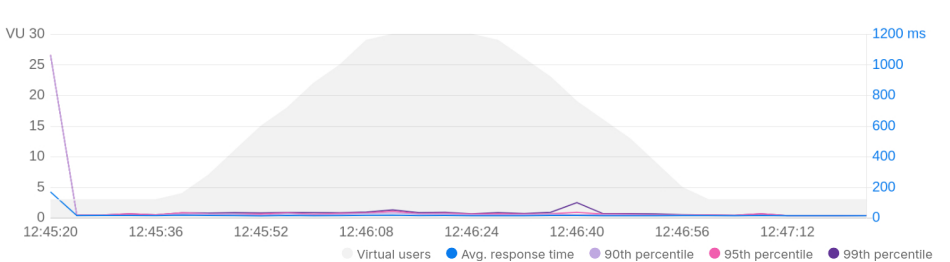
\includegraphics[width=1.0\textwidth]{immagini/peak30uv.png}
    \caption{Grafico Peak 30 VU}
    \label{fig:peak30uv}
\end{figure}

\begin{figure}[H] % <--- Forzato il posizionamento qui
    \centering
    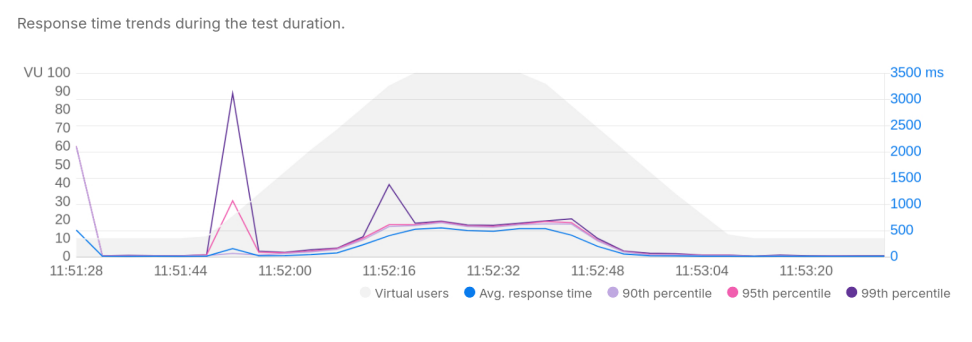
\includegraphics[width=1.0\textwidth]{immagini/peak100uv.png}
    \caption{Grafico Peak 100 VU}
    \label{fig:peak100uv}
\end{figure}

\subsubsection{Considerazioni Tecniche}

L'esecuzione dei test di carico a volumi di traffico reali ha permesso di delineare con maggiore precisione i limiti di scalabilità e la robustezza del backend sviluppato. L'analisi dei dati aggregati nelle tabelle \ref{tab:test_postman_portatile} e \ref{tab:test_postman_fisso} evidenzia i seguenti comportamenti del sistema:

\begin{itemize}
    \item \textbf{Efficienza in Condizioni Standard (Saturazione Bassa/Media):} Nello scenario a carico costante con 5 VU, il sistema risponde con un tempo medio estremamente ridotto ($\sim$21~ms). Questo valore, unito ai $\sim$32~ms registrati con 20 VU costanti, dimostra l'ottima efficienza della logica di routing e della gestione dei thread.
    
    \item \textbf{Scalabilità Lineare e Curve di Ramp-up:} I test di \textit{Ramp-up} lineare (fino a 5, 20 e 30 VU) mostrano un comportamento quasi ottimale, con tempi a regime stabili tra i $16\text{ ms}$ e i $18\text{ ms}$. Il server si dimostra capace di allocare dinamicamente le risorse necessarie man mano che nuove connessioni vengono stabilite, senza subire degradazioni prestazionali premature.
    
    \item \textbf{Analisi degli Scenari di Stress Avanzati (30 e 100 VU):} 
    Nel test \textit{Ramp-up up\&down} a 30 VU si nota un primo incremento del tempo a regime, che sale a $40\text{ ms}$. La vera e propria soglia di stress strutturale viene tuttavia raggiunta nello scenario a 100 VU (\textit{Ramp-up up\&down}): in questo caso il tempo medio globale si attesta a $268\text{ ms}$, ma subisce un raddoppio sensibile arrivando a $500\text{ ms}$ una volta raggiunto il pieno regime di carico.
    
    \item \textbf{Resistenza agli Spike:} 
    Lo \textit{Spike} a 20 VU mostra un tempo massimo di $4.0\text{ s}$, che sale linearmente a $7.0\text{ s}$ nello \textit{Spike} a 30 VU; anche nel \textit{Peak} a 100 VU in fase di salita è presente un tempo massimo di risposta di $3.0\text{ s}$. Questo incremento dei tempi di risposta massimi durante i picchi impulsivi evidenzia che il backend, pur non andando in \textit{crash}, soffre di un fenomeno temporaneo di \textit{saturazione delle risorse} quando riceve un numero anomalo di richieste improvvise, situazione che viene comunque assorbita superata la fase critica.
\end{itemize}

\section{Test di Sicurezza e Modello Zero Trust}

A completamento dell'analisi prestazionale, è stata condotta una batteria di test di sicurezza (eseguiti tramite una suite di test integrata nel cluster Docker) volti a verificare l'effettiva capacità dell'architettura Zero Trust di intercettare, valutare e neutralizzare pattern di attacco noti e comportamenti anomali. 

I test eseguiti hanno simulato sia attacchi frontali diretti contro il proxy esposto (Envoy), sia tentativi furtivi di movimento laterale diretti ai servizi interni, validando il funzionamento combinato del sistema di Intrusion Detection (Snort) e del decisore intelligente (AI Scorer).

\subsection{Scenari di Attacco Simulati}
La suite di test automatizzata ha replicato i seguenti scenari malevoli:
\begin{itemize}
    \item \textbf{SQL Injection (Mid-Level).} Simulazione di una query malevola all'endpoint delle API (\texttt{UNION SELECT * FROM users}), correttamente rilevata dalle regole Snort intermedie e bloccata (restituendo un errore 403 Forbidden).
    \item \textbf{Cross-Site Scripting (XSS).} Iniezione di uno script dannoso all'interno dei parametri di richiesta HTTP, parimenti neutralizzata dalla pipeline di sicurezza.
    \item \textbf{Utilizzo di Protocolli Obsoleti (Legacy TLS).} Invio di richieste di handshake SSLv3 forzate, le quali violano le policy di crittografia aggiornate e scatenano allarmi specifici a livello di rete.
    \item \textbf{Movimento Laterale Furtivo (Slowloris).} Per testare la resilienza alle minacce interne, il client ha bypassato volontariamente il proxy tentando una connessione diretta all'interfaccia dell'Orchestrator. Per eludere le rigide soglie volumetriche, l'attacco è stato condotto con la tecnica \textit{Slowloris}, trasmettendo un frammento di intestazione HTTP ogni due secondi, consumando le risorse senza destare allarmi di rete elementari.
\end{itemize}

\subsection{L'Intervento dell'AI Scorer}
Il banco di prova si è concluso con la verifica sul motore di intelligenza artificiale. A tale scopo è stata inviata una richiesta HTTP legittima (indirizzata a \texttt{/login}) e dotata di certificati crittografici validi, per innescare il flusso autorizzativo standard di Envoy verso l'Orchestrator.

Nonostante la richiesta risultasse formalmente valida, il sistema ha dimostrato un comportamento adattivo: l'AI Scorer ha analizzato la cronologia recente del client, che includeva i tentativi di attacco precedentemente simulati (tra cui il movimento laterale). Rilevando tali pattern anomali, il modello ha incrementato lo score di anomalia associato al client. Poiché il livello di rischio risultante ha superato le tolleranze consentite dalle policy in OPA, la richiesta è stata respinta preventivamente (HTTP 403 Forbidden).

Questi risultati confermano empiricamente che il sistema garantisce una validazione continua del comportamento, mitigando le minacce provenienti da entità compromesse prima che queste possano accedere alle risorse critiche dell'infrastruttura.
\end{document}